\documentclass[twocolumn]{sagej}

% Load basic packages
\usepackage{balance}		% to better equalize the last page
\usepackage{graphics}		% for EPS, load graphicx instead
\usepackage{times}			% comment if you want LaTeX's default font
\usepackage{url}			% llt: nicely formatted URLs
\usepackage{dblfloatfix}	% allow placement of a page-width figure at top or bottom of page

% llt: Define a global style for URLs, rather that the default one
\makeatletter
\def\url@leostyle{%
  \@ifundefined{selectfont}{\def\UrlFont{\sf}}{\def\UrlFont{\small\bf\ttfamily}}}
\makeatother
\urlstyle{leo}

\usepackage{tikz}
% Make sure hyperref comes last of your loaded packages,
% to give it a fighting chance of not being over-written,
% since its job is to redefine many LaTeX commands.
\usepackage[pdftex]{hyperref}

\newcommand{\modelfraction}{0.65}
\newcommand{\betweenmodels}{0.8cm}
\newcommand{\plotfraction}{0.85}
\newcommand{\pSim}{pSim}

% End of preamble. Here comes the document.
\begin{document}

\title{A PDEVS Simulator Supporting Multiple Synchronization Protocols: Implementation and Performance Analysis}

\author{Ben Cardoen\affilnum{1}, Stijn Manhaeve\affilnum{1}, Yentl Van Tendeloo\affilnum{1}, and Jan Broeckhove\affilnum{1}}

\affiliation{\affilnum{1}University of Antwerp, Belgium}

\corrauth{Yentl Van Tendeloo\\
University of Antwerp\\
Middelheimlaan 1\\
2020 Antwerp, Belgium}

\email{Yentl.VanTendeloo@uantwerpen.be}

\begin{abstract}
With the ever increasing complexity of simulation models, parallel simulation becomes necessary to perform simulation within reasonable time bounds.
The built-in parallelism of Parallel DEVS is often insufficient to tackle this problem on its own.
Several synchronization protocols have been proposed, each with their distinct advantages and disadvantages.
Due to the significantly different implementation of these protocols, most Parallel DEVS simulation tools are limited to only one such protocol.
In this paper, we present a Parallel DEVS simulator, grafted on C++11 and based on PythonPDEVS, supporting both conservative and optimistic synchronization protocols.
The simulator not only supports both protocols but also has the capability to switch between them at runtime.
We evaluate the performance gain obtained by choosing the most appropriate synchronization protocol.
A comparison is made to adevs in terms of CPU time and memory usage, to show that our modularity does not hinder performance.
We further allow for an external component to gather simulation statistics, on which runtime switching between the different synchronization protocols can be based.
Model allocation is also studied to see how our conservative and optimistic synchronization protocols are affected by good and bad allocations.

\end{abstract}

\maketitle
\begin{center}
Submission for the \textit{Special Issue of Simulation: SpringSim 2016 special issue}.
\end{center}

%todo macro pSim
\section{Introduction}
\label{sec:1-introduction}
\textsf{DEVS}~\cite{ClassicDEVS} is a popular formalism for modelling complex dynamic systems using a discrete-event abstraction.
In fact, it can serve as a simulation ``assembly language'' to which models in other formalisms can be mapped~\cite{DEVSbase}.
A number of tools have been constructed by academia and industry that allow the modelling and simulation of \textsf{DEVS} models.

But with the ever increasing complexity of simulation models, parallel simulation becomes necessary to perform the simulation within reasonable time bounds.
And while \textsf{Parallel DEVS}~\cite{ParallelDEVS} was introduced to increase parallelism, this is often insufficient.
Several synchronization protocols from the discrete event simulation community~\cite{FujimotoBook} have been applied to \textsf{DEVS} simulation.
While several parallel \textsf{DEVS} simulation kernels exist, they are often limited to a single synchronization protocol.
The reason for different synchronization protocols, however, is that their distinct nature makes them applicable in different situations, each outperforming the other in specific models.
The applicability of parallel simulation capabilities of current tools is therefore limited.

This paper introduces DEVS-Ex-Machina\footnote{\url{https://bitbucket.org/bcardoen/devs-ex-machina}} (``dxex''), our simulation tool which offers multiple synchronization protocols: no synchronization (sequential execution), conservative synchronization, or optimistic synchronization.
The selected synchronization protocol is transparent to the simulated model: users should merely determine, which protocol they wish to use.
Users who simulate a wide variety of models, with different ideal synchronization protocols, can simply run the same model with different synchronization protocols.
We investigate in this paper how model allocation and uncertainty determine the choice between synchronization protocols. 
The synchronization overhead is demonstrated by reducing the computational load of a model to near zero. 

Our tool is based on PythonPDEVS, but implemented in C++11 for increased performance, using features from the new C++14 standard when possible.
Unlike PythonPDEVS dxex only supports multicore parallelism.

We implemented a model that, depending on a single parameter, changes its ideal synchronization protocol. We demonstrate using several models the factors influencing the performance under a given synhronization protocol.
Dxex, then, is used to compare simulation using exactly the same tool, but with a varying synchronization protocol. With dxex users can always opt to use the fastest protocol available.
To verify that our flexibility does not counter performance, we compare to adevs, currently one of the fastest \textsf{DEVS} simulation tools available~\cite{PythonPDEVS,DEVSSurvey}.

% Switching and statistics
Dxex offers visualization of the simulation and in depth statistics. A modeller can then make a more informed decision on which synchronization protocol to use or even intervene during simulation and request a switch between protocols. 

%Usage of Hyperref with hardcoded label is hardly ideal, but ~\ref doesn't work if the layout disables numbered sections, so a hack is needed. The alternative is \nameref but that isn't all that readable.
The remainder of this paper is organized as follows:
Section~\hyperref[sec:2-background]{2} introduces the necessary background on synchronization protocols.
Section~\hyperref[sec:3-features]{3} elaborates on our design that enables this flexibility.
In Section~\hyperref[sec:4-performance]{4}, we evaluate performance of our tool by comparing its different synchronization protocols, and by comparing to adevs.
Related work is discussed in Section~\hyperref[sec:5-related-work]{5}.
Section~\hyperref[sec:6-conclusion]{6} concludes the paper and gives future work.


\section{Background}
\label{sec:2-background}
This section briefly introduces the two synchronization protocols used by dxex: conservative and optimistic synchronization.

\subsection{Conservative Synchronization}
The first synchronization protocol we introduce is \textit{conservative synchronization}~\cite{FujimotoBook}.
In conservative synchronization, a node progresses independent of all other nodes, up to the point in time where it can guarantee that no causality errors happen.
When simulation reaches this point, the node blocks until it can guarantee a new time until which no causality errors happen.
In practice, this means that all nodes are aware of the current simulation time of all other nodes, and the time it takes an event to propagate (called \textit{lookahead}).
Deadlocks can occur due to a dependency cycle of models.
Multiple algorithms are defined in the literature to handle both the core protocol, as well as resolution schemes to handle or avoid the deadlocks~\cite{FujimotoBook}.

The main advantage of conservative synchronization is its low overhead if the lookahead is high.
Each node then simulates in parallel, and sporadically notifies other nodes about its local simulation time.
The disadvantage, however, is that the amount of parallelism is explicitly limited by the lookahead.
If a node can influence another (almost) instantaneously, no matter how rarely it occurs, the amount of parallelism is severely reduced.
The user is required to define the lookahead, using knowledge about the model's behaviour.
Defining lookahead is not always a trivial task if there is no detailed knowledge of the model.
Even slight changes in the model can change to the lookahead, and can therefore have a significant influence on simulation performance.

\subsection{Optimistic Synchronization}
A completely different synchronization protocol is \textit{optimistic synchronization}~\cite{TimeWarp}.
Whereas conservative synchronization would prevent causality errors at all costs, optimistic synchronization will allow them to happen, but correct them afterwards.
Each node is allowed to progress in simulated time as much as possible, without taking note of the state of any other node.
When an event arrives at a node, which is already further in simulated time, the node will have to roll back its state to right before the event would normally have to be processed.
As the simulation time is now rolled back to before the event is processed, the event can simply be processed as if no causality error ever occured.

Rolling back the simulation time requires the node to store past model states, such that they can be restored later on.
Furthermore, all incoming and outgoing events need to be stored as well.
Incoming events need to be passed to the models again, when the correct simulation time has again been reached, and outgoing events need to be cancelled, as potentially a different series of output events would normally have been generated.
Cancelling events, however, can cause further rollbacks, as the receiving node might also have to roll back its state.
In practice, a single causality error could have significant repercussions on the complete simulation.

Further changes are required for unrecoverable operations, such as I/O (\textit{e.g.}, tracing, writing to file, printing output) and memory management.
Lightweight algorithms are still required to determine the lower bound of all simulation times, through the computation of a \textit{Global Virtual Time} (GVT).

The main advantage is that performance is not limited by a small lookahead, caused by a very infrequent event.
If an (almost) instantaneous event occurs rarely, performance will only be impacted if it occurs, and not at every simulation step.
The main disadvantage is unpredictable performance and arbitrary cost of rollbacks due to the propagation of causality errors.
If rollbacks occur frequently, simulation quickly becomes slow, as the overhead of the recovery mechanisms becomes significant.
Apart from overhead in CPU time, a significant memory overhead is present: all intermediate states qre stored up to a point where it can be considered \textit{irreversible}.

While optimistic synchronization does not explicitly depends on the lookahead, simulation performance is still bound by the lookahead implicitly.


\section{DEVS-Ex-Machina}
\label{sec:3-features}
Historically, dxex is based on PythonPDEVS~\cite{PythonPDEVS}.
Python is a good language for prototypes, but performance has proven insufficient to compete with other simulation kernels~\cite{MasterThesis}.
Dxex is a C++11-based implementation of PythonPDEVS, but implements only a subset of PythonPDEVS, while making some of its own additions.
So while the feature set is not too comparable, the architectural design, core simulation algorithm, and optimizations, are highly similar.

We will not make a detailed comparison with PythonPDEVS here, but only mention some supported features.
Dxex supports, similarly to PythonPDEVS, the following features: direct connection~\cite{SymbolicFlattening}, \textsf{Dynamic Structure DEVS}~\cite{DSDEVS}, termination conditions, and a modular tracing and scheduling framework~\cite{PythonPDEVS}.
But whereas PythonPDEVS only supports optimistic synchronization, dxex support multiple synchronization protocols (though only in parallel).
This is in line with the design principle of PythonPDEVS: allow users to pass performance hints to the simulation kernel.
In our case, a user can pass the simulation kernel sets the synchronization protocol to be used for this model.
Our implementation in C++11 also allows for optimizations which were plainly impossible in an interpreted language.

Since there is no universal \textsf{DEVS} model standard, dxex models are incompatible with PythonPDEVS and vice versa.
This is due to dxex models being grafted on C++11, whereas PythonPDEVS models are grafted on Python.

In the remainder of this section, we will elaborate on our prominent new feature: support for multiple synchronization protocols within the same simulation tool, which are offered transparently to the model.

\subsection{Synchronization protocols}
We previously explained the existence of different synchronization protocols exist, each optimized for a specific kind of model.
As no single synchronization protocol is ideal for all models, a general purpose simulation tool should support multiple protocols.
Currently, most parallel simulation tools choose only a single synchronization protocol due to the inherent differences between protocols.
An uninformed choice on which one to implement is insufficient, as performance will likely be bad.
We argue that a real general purpose simulation tool should support sequential, conservative, and optimistic synchronization, as is the case for dxex.

These different protocols relate to three different model characteristics.
Conservative synchronization for when high lookahead exists between different nodes, and barely any blocking is necessary.
Optimistic synchronization for when lookahead is unpredictable, or there are rare (almost) instantaneous events.
Finally, sequential simulation is still required for models where parallelism is bad, where all protocols actually slow down simulation.

\subsubsection{Sequential}
Our sequential simulation algorithm is very similar to the one found in PythonPDEVS, including many optimizations.
Minor modifications were made, though, such that it can be overloaded by different synchronization protocol implementations.
This way, the \textsf{DEVS} simulation algorithm is implemented once, but parts can be overridden as needed.
In theory, more synchronization protocols (\textit{e.g.}, other algorithms for conservative synchronization) can be added without altering our design.

An overview of dxex's design is given in Figure~\ref{fig:class_diagram}.
It shows that there is a simulation \texttt{Core}, which simulates the \texttt{AtomicModel}s connected to it.
The superclass \texttt{Core} is merely the sequential simulation core, but can be used as-is.
Subclasses define specific variants, such as \texttt{ConservativeCore} (conservative synchronization), \texttt{OptimisticCore} (optimistic synchronization), and \texttt{DynamicCore} (\textsf{Dynamic Structure DEVS}).

\begin{figure}
    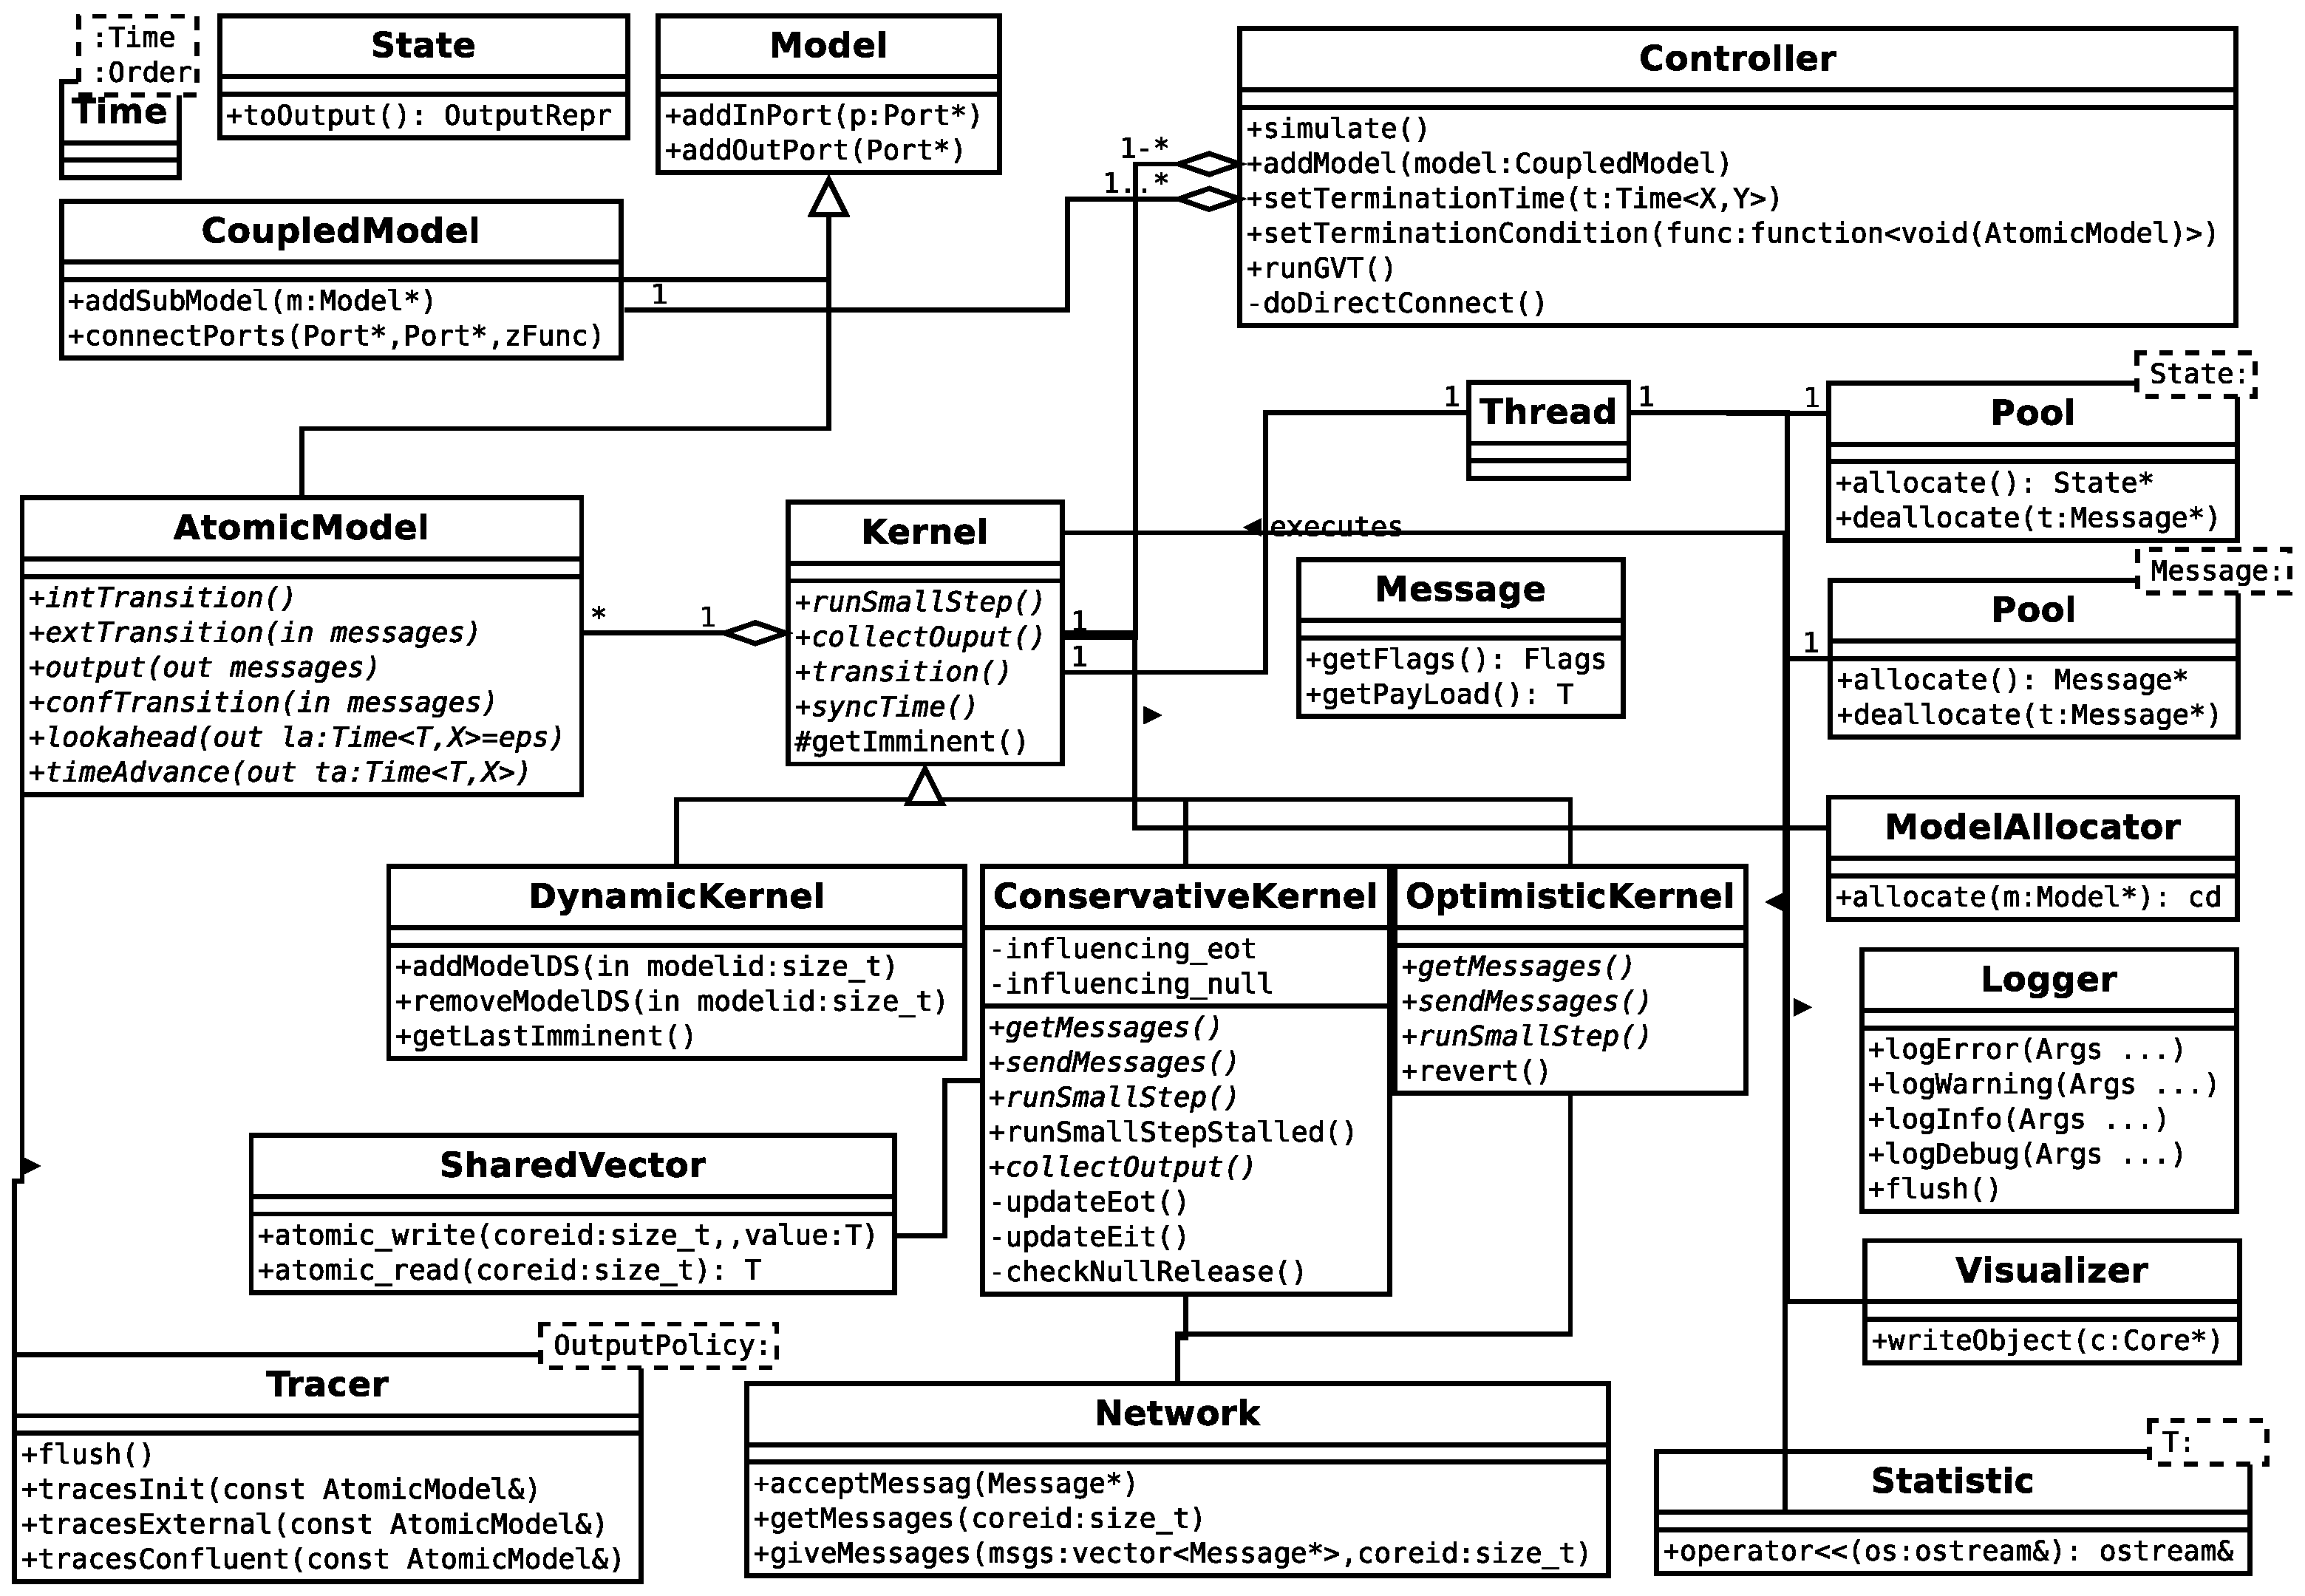
\includegraphics[width=\columnwidth]{fig/cores_class_diagram.eps}
	\caption{Dxex kernel design.}
	\label{fig:class_diagram}
\end{figure}

\subsubsection{Conservative}
For conservative synchronization, each node must determine the nodes it is influenced by.
Each model needs to provide a lookahead function, which determines the lookahead depending on the current simulation state.
Within the returned time interval, the model promises not to raise an event.
A node aggregates this information to computes its earliest output time (EOT).
This value is written out in shared memory, where it can be read out by all other nodes.

Reading and writing to shared memory is done through the use of the new C++11 synchronization primitives.
Whereas this was also possible in previous versions of the C++ standard, by falling back to non-portable C functions, it was not a part of the C++ language standard.
C++11 further allows us to make the implementation portable, as well as more efficient: the compiler might know of optimizations specific to atomic variables.

\subsubsection{Optimistic}
For optimistic synchronization, each node must be able to roll back to a previous point in time.
This is often implemented through the use of state saving.
This needs to be done carefully in order to avoid unnecessary copies, and minimize the overhead.
We use the default: explicitly save each and every intermediate state.
Mattern's algorithm~\cite{mattern} is used to determine the GVT, as it runs asynchronously and uses only $2n$ synchronization messages.
Once the GVT is found, all nodes are informed of the new value, after which fossil collection is performed, and irreversible actions are committed.

The main problem we encountered in our implementation is the aggressive use of memory.
Frequent memory allocation and deallocation caused significant overheads, certainly when multiple threads do so concurrently.
This made us switch to the use of thread-local (using \texttt{tcmalloc}) memory pools.
Again, we made use of specific new features of C++11, that were not available in Python, or even previous versions of the C++ language standard.

\subsection{Transparency}
We define simulation kernel transparency as having a single model, which always can be executed on each supported synchronization kernel, without any modifications.
User should thus only provide one model, implemented in C++11, which can be either using sequential execution, using conservative synchronization, or using optimistic synchronization.
Switching between simulation kernels is as simple as altering the simulation termination time.
The exception is conservative synchronization, where a lookahead function is required, which is not used in other synchronization kernels.
Two options are possible: either a lookahead function must always be provided, even when it is not required and possibly not used, or we use a default lookahead function if none is defined.

Always defining a lookahead function might seem redundant, especially if users will never use conservative synchronization.
Especially since defining the lookahead is often non-trivial and dependent on intricate model details.
The more attractive option is for the simulation tool to provide a default lookahead function, such that simulation can run anyway, but maybe not at peak performance.
%Depending on the model, simulation performance might still be faster than sequential simulation. 

Defining a lookahead function is therefore recommended in combination with conservative synchronization, but is not a necessity, as a default of $epsilon$ can be used otherwise.


\section{Performance Evaluation}
\label{sec:4-performance}
% DESIGN OF MODELS
\section{Atomic models}

\section{Coupled models}

% SEQUENTIAL
\subsection{Sequential Simulation}
We start by evaluating sequential simulation performance, in order to obtain a baseline for our comparison of parallel simulation performance.

\subsubsection{Queue}
\label{4-seq-Queue}
% explain what we did: fixed number of models (400, 600 & 800), increasing depth
For the first benchmark, we tested the effect of hierarchical complexity of the model in the performance of the simulator.
A set of three tests was performed, where each test has the same number of models but an increasing depth.
The results can be seen in Figure~\ref{fig:Queue_benchmark_seq}.
Since dxex symbolically flattens the model, there is no performance hit when the depth is increased.
The overhead of running the directconnect algorithm is one time only and negligible when the end time of the simulation is sufficiently large.
Adevs on the other hand does suffer from the increased depth.
With every new hierarchical layer, routing an event from one atomic model to the next becomes more expensive, resulting in an increase in runtime.
\begin{figure}
	\center
	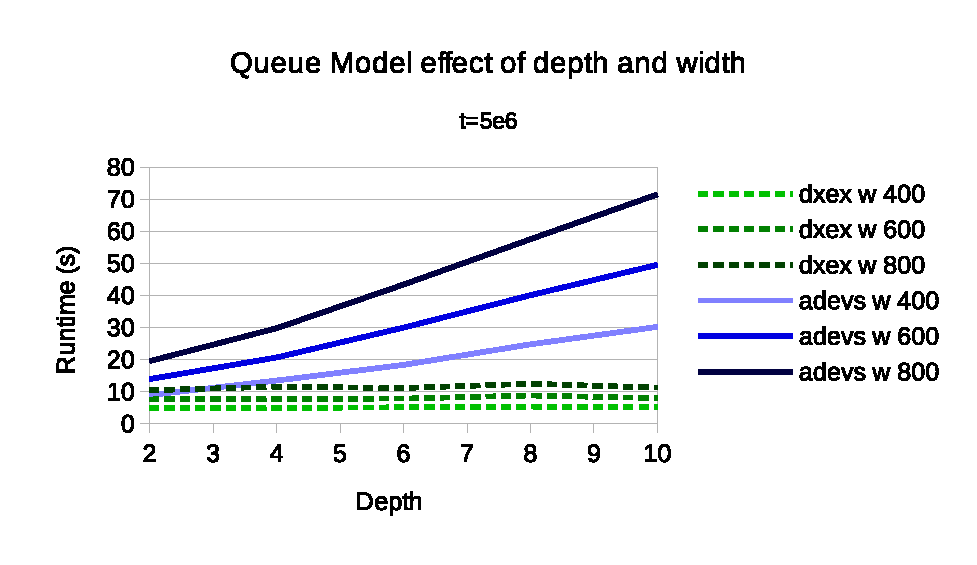
\includegraphics[width=\columnwidth]{fig/queue_fixed_sequential.eps}
	\caption{Queue benchmark results for sequential simulation.}
	\label{fig:Queue_benchmark_seq}
\end{figure}

\subsubsection{Interconnect}
\label{4-seq-Interconnect}
In the Interconnect model, we increase the number of atomic models, thus quadratically increasing the number of couplings and the number of external transitions.
As can be seen in Figure~\ref{fig:Interconnect_benchmark}, adevs outperforms dxex by a fair margin.
Analysis showed that this is caused by the high amount of events: event creation is much slower in dxex than it is in adevs, despite dxex's use of memory pools.
To shield the user from threading and deallocation concerns dxex provides an event superclass from which the user can derive to create a specialized event type.
Copying and deallocation semantics and tracing are solved by the kernels at a runtime cost in simulations where event frequency is very high.
Profiling the benchmarks clearly shows the increasing cost of output generation and deallocation as the determining factor in the gap in performance.
We refer the interested reader to the dxex \hyperref{https://bitbucket.org/bcardoen/devs-ex-machina}{}{repo}{repository} for the profiling call graphs for the different benchmarks.

\begin{figure}
	\center
	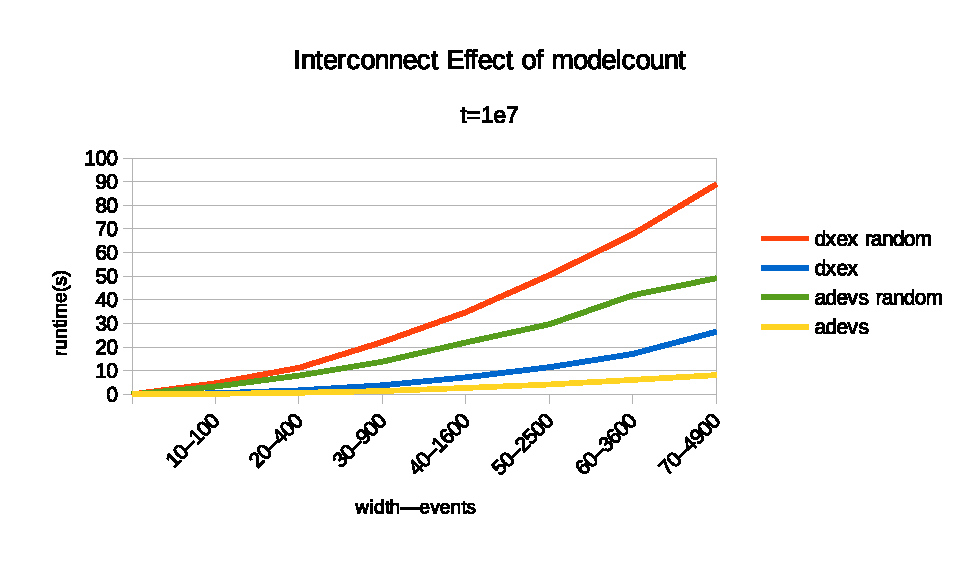
\includegraphics[width=\columnwidth]{fig/interconnect_sequential.eps}
	\caption{Interconnect benchmark results for sequential simulation.}
	\label{fig:Interconnect_benchmark}
\end{figure}

\subsubsection{PHold}
\label{4-seq-PHold}
The PHold model is very similar to the Interconnect model.
The biggest difference is that the amount of messages sent is much lower.
The number of events scales linear with the number of models, not quadratic.
Figure~\ref{fig:Phold_benchmark} shows that the performance of dxex and adevs are very close to each-other, with adevs slightly outperforming dxex.
\begin{figure}
	\center
	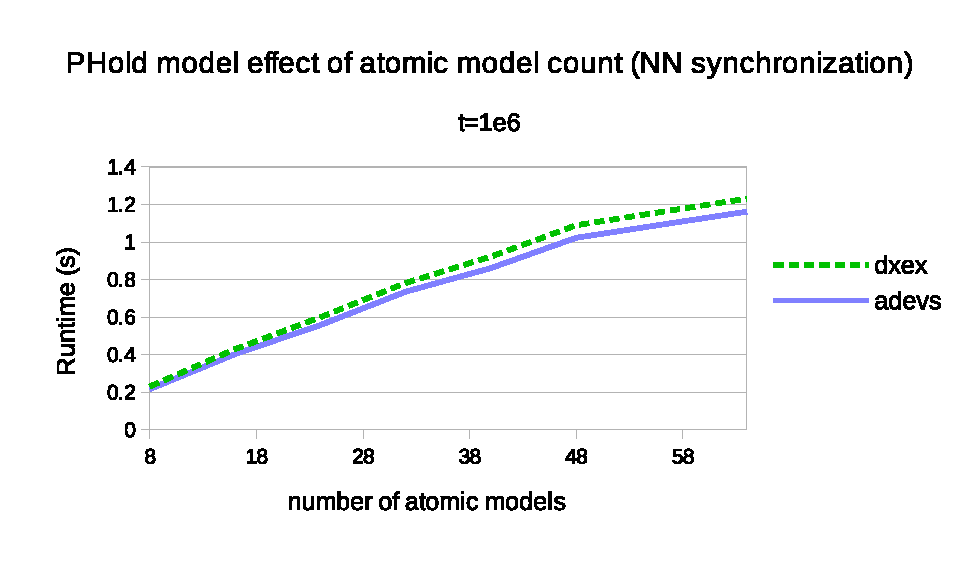
\includegraphics[width=\columnwidth]{fig/phold_sequential.eps}
	\caption{PHold benchmark results for sequential simulation.}
	\label{fig:Phold_benchmark}
\end{figure}


% PARALLEL
\subsection{Parallel Simulation}

% The good
\subsubsection{Queue}
\paragraph*{Allocation}
The Queue model is one single chain of models. Each kernel gets one connected part of this chain. The result is that the kernels themselves also form a chain where events only travel in one direction.

\paragraph*{Strong and Weak Scaling}
Figure~\ref{fig:Queue_plot_strong} shows the speedup compared to dxex sequential for a fixed problem size. As the amount of kernels increases, the optimistic kernel quickly becomes the worst choice. The difference between dxex conservative and adevs becoming smaller. The same effect can be seen for weak scaling in Figure~\ref{fig:Queue_plot_weak}.\\
In Figure \ref{fig:Queue_allocation} the allocation of the Queue model is visualized. This trace allows us to demonstrate the benchmark results and explain why optimistic is not ideal for such a chain topology as present in Queue. Kernel 2 is dependent on events from kernels 0 and 1 but by definition of the optimistic synchronization protocol it will simulate ahead without waiting for events it depends on. Any simulation it performs will have to be reverted as soon as events from kernels 0 and 1 arrive. When kernel 2 reverts, kernel 3 will inevitably have to revert as well since most of the events it received from kernel 2 are invalidated and marked as such by antimessages. This leads to severe performance degradation, with an increasing probability of cascading reverts as the number of kernels and models per kernels increases.
The speedup of adevs is always in comparison with the runtime of the corresponding dxex sequential benchmark.
\begin{figure}
	\center
	
	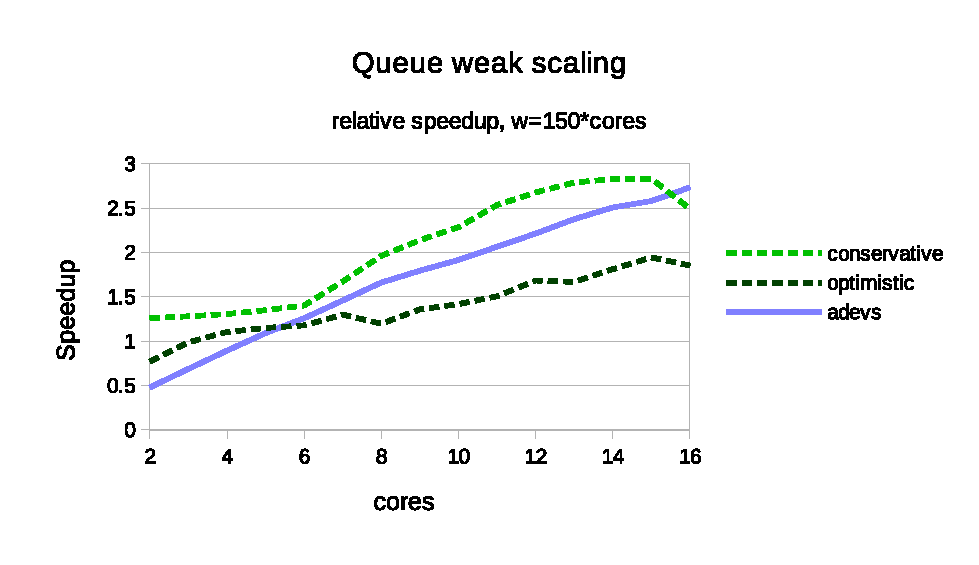
\includegraphics[width=\modelfraction\columnwidth]{fig/queue_fixed_weak_speedup.eps}
	\caption{Queue model weak scaling speedup compared to dxex sequential.}
	\label{fig:Queue_plot_weak}
	
	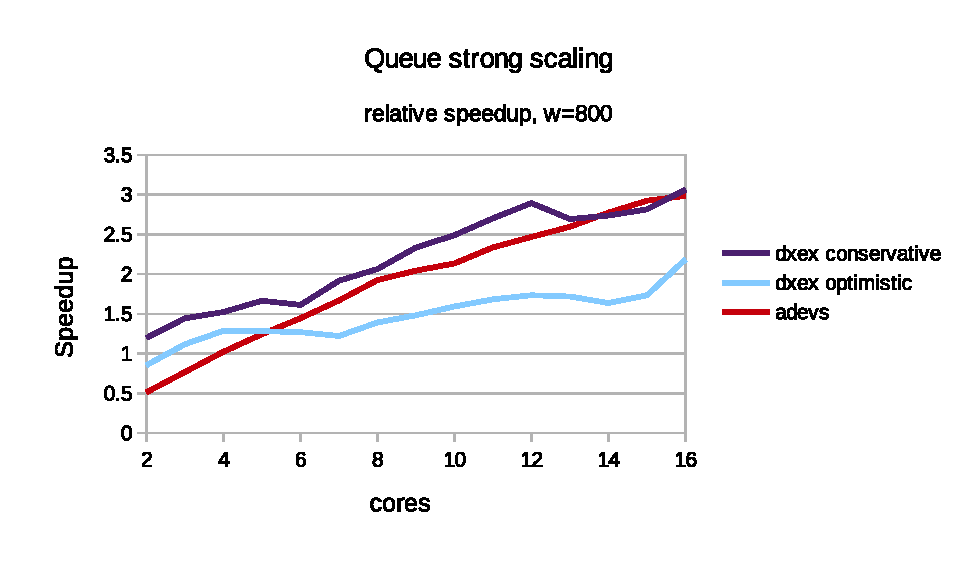
\includegraphics[width=\modelfraction\columnwidth]{fig/queue_fixed_strong_speedup.eps}
	\caption{Queue model strong scaling speedup compared to dxex sequential.}
	\label{fig:Queue_plot_strong}
		
\end{figure}

\begin{figure}
	\center
	
	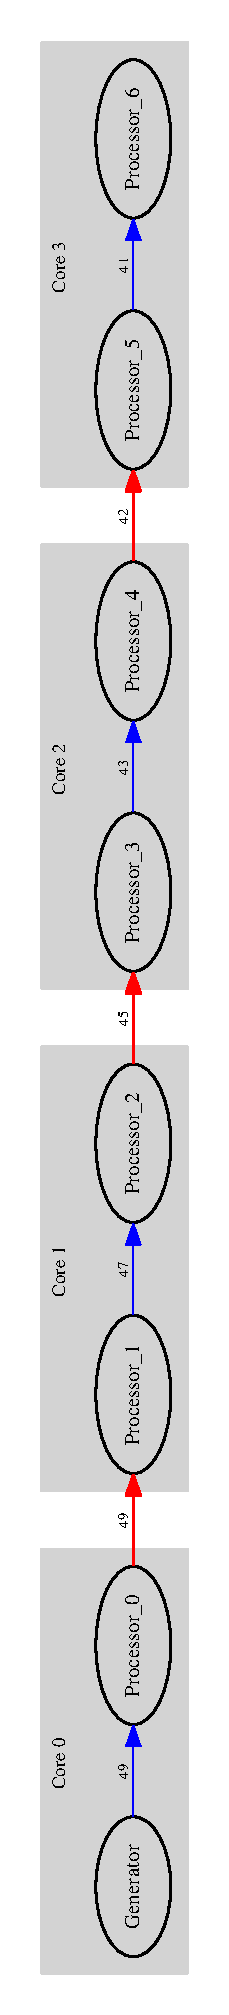
\includegraphics[width=\modelfraction\columnwidth, height=8cm, keepaspectratio, angle=-90 ]{fig/queue_allocation.eps}
	\caption{Queue model (d=2, w=7, t=5000, random timeadvance) allocation and simulation trace across 4 kernels.}
	\label{fig:Queue_allocation}
	
\end{figure}

% The really bad
\subsubsection{Interconnect}\label{subsec:parallelinterconnect}
In the Interconnect model, we determine how broadcast communication is supported across multiple nodes.
The number of models is now kept constant at eight.
Results are shown in Figure~\ref{fig:interconnect_benchmark_parallel}.
When the number of nodes increases, performance decreases due to increasing contention in conservative simulation and an increasing number of of rollbacks in optimistic simulation.
All models depend on each other and have no computational load whatsoever, negating any possible performance gain by executing the simulation in parallel.
In Interconnect there is no allocation scheme possible that avoids cyclic dependencies between simulation kernels, as shown in the trace \ref{fig:interconnect_allocation_parallel} of a simulation with 4 models. Such a cycle forces sequential operation of the kernels with no speedup possible.

\begin{figure}
	\center
	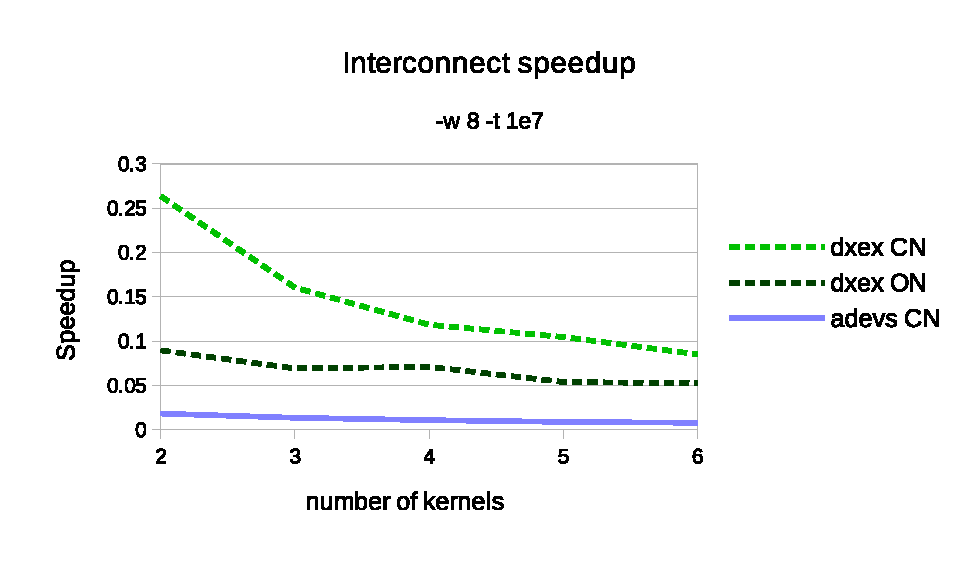
\includegraphics[width=\plotfraction\columnwidth]{fig/interconnect_parallel.eps}
	\caption{Interconnect benchmark results for parallel simulation.}
	\label{fig:interconnect_benchmark_parallel}
\end{figure}
\begin{figure}
	\center
	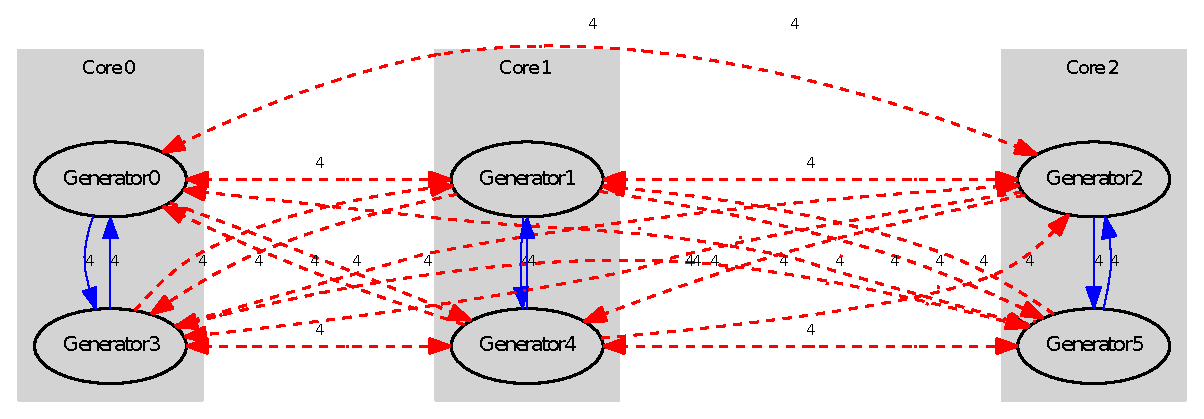
\includegraphics[width=\plotfraction\columnwidth]{fig/interconnect_parallel_allocation.eps}
	\caption{Interconnect parallel simulation trace for 6 models on 3 kernels.}
	\label{fig:interconnect_allocation_parallel}
\end{figure}

% The okayish
\subsubsection{Phold}
% Same cause, different results
In the Phold model, we first investigate the influence of the percentage of remote events on the speedup. A remote event in this context is an event that is sent from a model on one kernel to a model on another simulation kernel.
When remote events are rare, optimistic synchronization rarely has to roll back, thus increasing performance.
With more common remote events, however, optimistic synchronization quickly slows down due to frequent rollbacks.
Conservative synchronization, on the other hand, is mostly unconcerned with the number of remote events: the mere fact that a remote event can happen, causes it to block and wait.
Even though a single synchronization protocol is always ideal in this case, it already shows that different synchronization protocols respond differently to a changing model.
Adevs is significantly slower during conservative synchronization.
Analysis of profiling callgraphs shows that exception handling in adevs is the main cause. 
To keep the models equivalent, the adevs version does not provide the \{begin,end\}Lookahead methods, which accounts for the exception handling. These functions require the user to implement a state saving in contrast to PythonPDEVS and dxex's optimistic kernels which handle this inside the kernel. We feel this would lead to an unfair comparison as we would like to keep the models synchronization-agnostic across all benchmarks.

\begin{figure}
    \center
    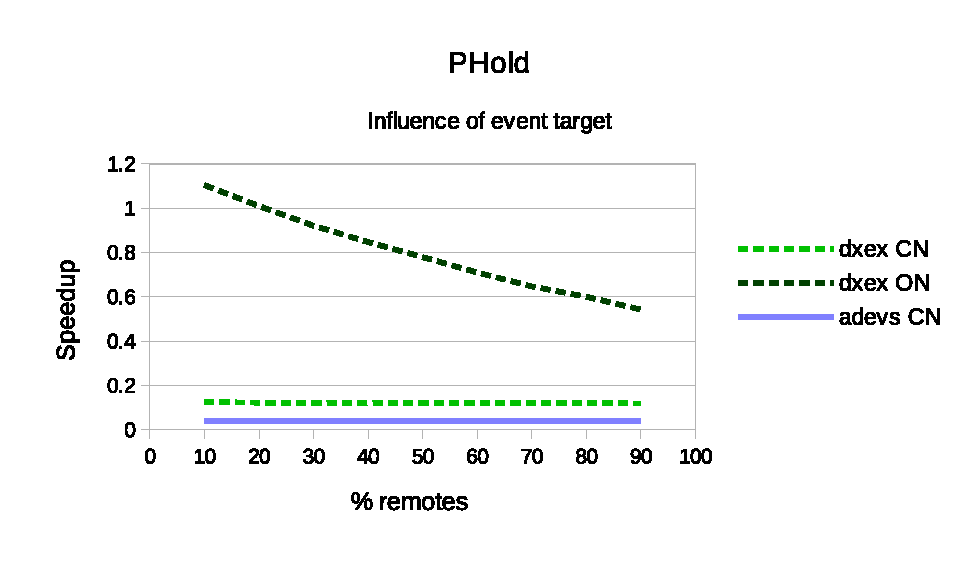
\includegraphics[width=\plotfraction\columnwidth]{fig/phold_remotes.eps}
    \caption{Phold benchmark results for parallel simulation using four kernels, four atomics per node, with varying percentage of remote events.}
\end{figure}
\begin{figure}
	\center
	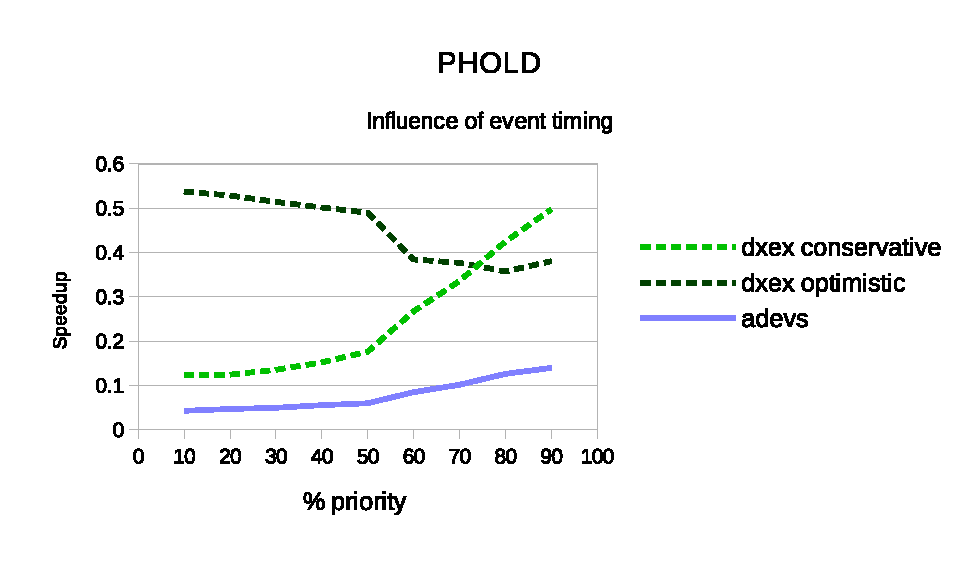
\includegraphics[width=\plotfraction\columnwidth]{fig/phold_priority.eps}
	\caption{Phold benchmark results for parallel simulation using four kernels, with varying amount of high-priority events.}
	\label{fig:phold_priority}
\end{figure}
\begin{figure}
	\center
	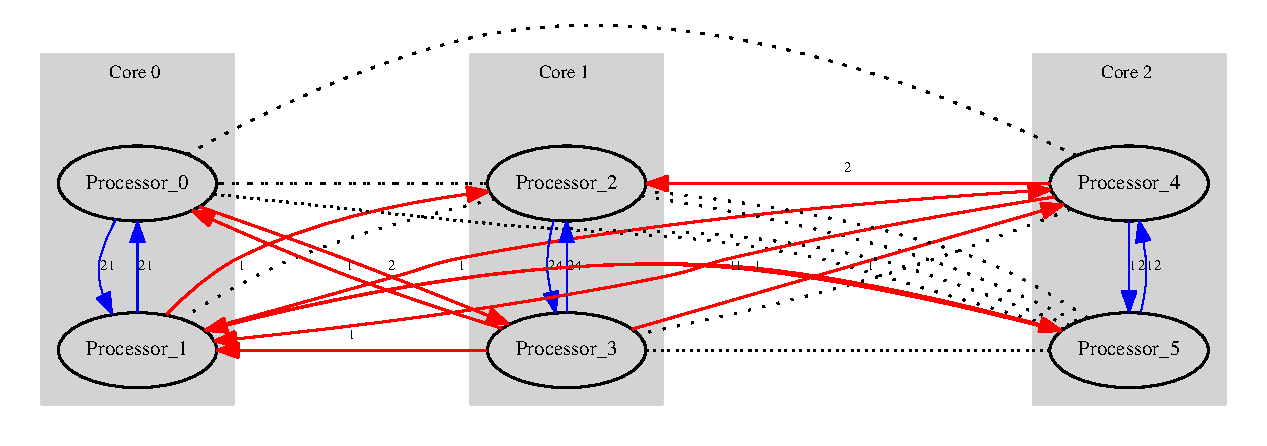
\includegraphics[width=\plotfraction\columnwidth]{fig/phold_parallel_allocation.eps}
	\caption{Phold benchmark trace for parallel simulation using three kernels.}
	\label{fig:phold_allocation}
\end{figure}

We slightly modified the Phold benchmark, to include high-priority events.
Contrary to normal events, high-priority events happen almost instantaneously, restricting lookahead to a very small value.
Even when normal events occur most often, conservative synchronization always blocks until it can make guarantees.
Optimistic synchronization, however, simply goes forward in simulation time and rolls back when these high-priority events happen.
This situation closely mimics the case made in the comparison between both synchronization algorithms by~\cite{FujimotoBook}.
In Figure \ref{fig:phold_allocation} it is clear that in Phold it is possible for dependency cycles to form between kernels which as we have shown in Interconnect degrades performance for both optimistic and conservative. This is also the cause of the sublinear speedup observed in our Phold benchmark.

Figure~\ref{fig:phold_priority} shows how simulation performance is influenced by the fraction of these high-priority events.
If barely any high-priority events occur, conservative synchronization is penalized due to its excessive blocking, which often turned out to be unnecessary.
When many high-priority events occur, optimistic synchronization is penalized due to its mindless progression of simulation, which frequently needs to be rolled back.
Results show that there is no single perfect synchronization algorithm for this model: depending on configuration, either synchronization protocol might be better.


\subsection{Comparison with PDEVS}
In this section we contrast the speedup between the original PDEVS algorithm and the synchronization protocols. 
Note that the PDEVS algorithm and the synchronization protocols are complementary in \textit{dxex}, not exclusive. 
Following the theoretical analysis published in ~\cite{amdahlpdevs} a comparison between PDEVS and the synchronization protocols was warranted. 
We compare the ideal scenario for PDEVS where all events are concurrent with a scenario where events are random.
In this work we do not consider the distribution of events, introducing a random number generator as we will show in this work can mask performance results. 
By limiting ourselves to the best and worst case scenario we demonstrate the capabilities and limitations of both approaches.
The influence of the computational load of the transition functions is a second factor we investigate in this section.
We are interested in scenarios where PDEVS and the synchronization protocols can complement each other in addition to observing their speedup in isolation.
The benchmarks are run on the same hardware as our previous results, a 8 x AMD Opteron(TM) Processor 6274 machine with 8 cores per cpu (64 cores) and 192 GB RAM. 
The benchmarks use a maximum of 16 threads to be divided between PDEVS , conservative or optimistic. 

\paragraph{Model}
As shown in the previous section, when most models are dependent on each other across kernels there is no speedup obtainable by either optimistic or conservative. 
We therefore opted to use the \textit{Queue} model in this benchmark, with depth 4 and width 300.
The effect of combining 4 synchronized kernels with each 4 threads for PDEVS is contrasted with 16 threads for PDEVS and 16 kernels for conservative and optimistic.  
This allows us to observe which is more efficient in obtaining a speedup.
We simulate a computational load by a call to sleep in the transition functions set at 5ms. 

\paragraph{Concurrent events}
First we create the ideal scenario for PDEVS, all events are concurrent with a significant computational load in the transition functions. 

In figure \ref{fig:pdevs_plot_fixed_sleep} we observe that PDEVS obtains a speedup approaching 8. 
Conservative and optimistic are run first with 16 kernels, then with 4 kernels having 4  PDEVS threads each. 
The resulting speedup is half of that obtained of the sequential kernel with 16 PDEVS threads.

\paragraph{Random events}
Random events allow us to demonstrate the overhead of PDEVS. The probability that events are concurrent is strongly reduced.
The transition function has the same computational load as in the previous configuration. 
The results in figure \ref{fig:pdevs_plot_random_sleep} demonstrate that the overhead in the sequential DPEVS kernel is negligible. In contrast both conservative and optimistic suffer a significant slowdown when combined with PDEVS.
We clearly see that conservative and optimistic outperform the sequential kernels in this scenario, complementing the synchronized kernels with PDEVS is not warranted here.

\paragraph{Computational load}
When we remove the computational load we isolate the overhead of the parallelism. 
In this paper we are mainly interested in this overhead which is otherwise masked by adding a computational cost to the transition functions. 
All the benchmarks in this work are run with a near negligible computational load in the transition functions for this purpose.
If a parallel speedup can be obtained in a simulation model without any load in the transition function this will translate in a higher speedup with an increased load, as this load can then be spread over kernels or threads.
Although this configuration has only concurrent events the overhead of the synchronization is severe. 
The runtime cost of this overhead is extreme in the sequential kernel. 
The synchronized kernels are impacted less by the overhead of the PDEVS algorithm.
 
\paragraph{Discussion}
In \textit{dxex} PDEVS and the two synchronization protocols are complementary. The user is not forced to choose between either but can divide the capabilities of his machine over both approaches.
While PDEVS can offer a significant speedup we see that to offer this speedup the concurrency of events must be significant in combination with a high computational load in the transition functions. 
We measure the overhead introduced by PDEVS to give practitioners insight into which model can benefit from which paradigm.
The overhead of the synchronization protocols in specific scenarios  is shown in the previous section.
For a given model it is difficult to predict the concurrency of events, although the computational load of a transition function can be approximated.
In these benchmarks we show which configurations can lead to a speedup for PDEVS or the synchronization protocols in isolation or combination.
In \citep{amdahlpdevs} a theoretical bound is defined for the maximum speedup obtained by PDEVS. 
Our tool flattens the hierarchy of the coupled models


\begin{figure}
	\center
	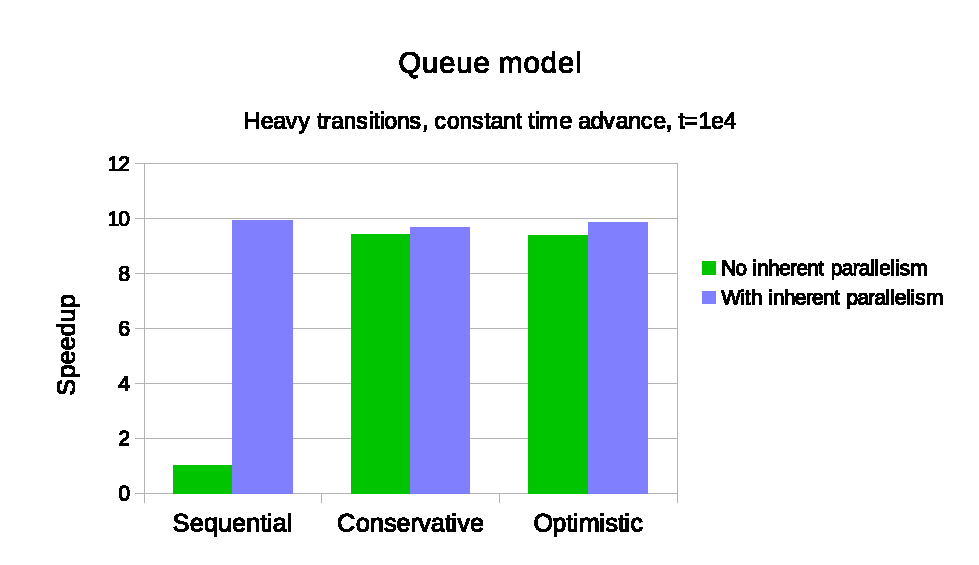
\includegraphics[width=\columnwidth]{fig/pdevs_fixed_sleep.eps}
	\caption{Queue speedup benchmark for PDEVS and synchronization with maximal concurrent events and significant computational load}
	\label{fig:pdevs_plot_fixed_sleep}
\end{figure}

\begin{figure}
	\center
	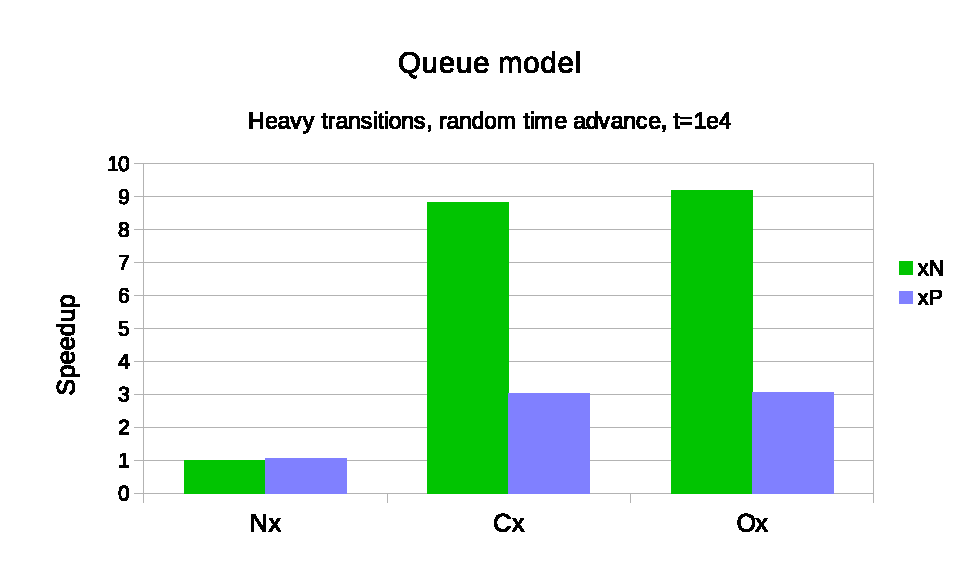
\includegraphics[width=\columnwidth]{fig/pdevs_random_sleep.eps}
	\caption{Queue speedup benchmark for PDEVS and synchronization with randomized events and significant computational load}
	\label{fig:pdevs_plot_random_sleep}
\end{figure}

\begin{figure}
	\center
	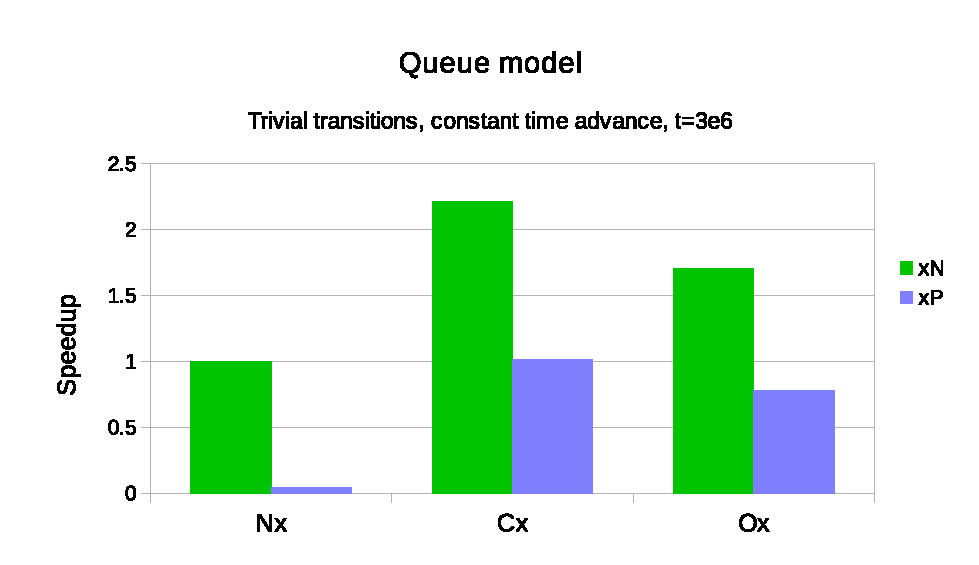
\includegraphics[width=\columnwidth]{fig/pdevs_no_sleep.eps}
	\caption{Queue speedup benchmark for PDEVS and synchronization with maximal concurrent events and trivial computational load}
	\label{fig:pdevs_plot_no_sleep}
\end{figure} 

\subsection{Memory Usage}
Apart from simulation execution time, memory usage during simulation is also of great importance.
While execution time only becomes a problem if it takes way too long, coming short only a bit of memory can make simulation unfeasible.
We therefore also investigate memory usage of different synchronization protocols, and again compare to adevs.

We do not tackle the problem of states that become too large for a single machine to hold.
This problem can be mitigated by distribution over multiple machines, which neither dxex or adevs support.

\subsubsection{Remarks}
Both dxex and adevs use \texttt{tcmalloc} as memory allocator, allowing for thread-local allocation.
Additionally, dxex uses memory pools to further reduce the frequency of expensive system calls (\textit{e.g.}, malloc and free).
\texttt{tcmalloc} only gradually releases memory back to the OS, whereas our pools will not do so at all.
Due to our motivation for memory usage analysis, we will only measure peak allocation in maximum resident set size as reported by the OS.

\subsubsection{Results}
Figure~\ref{fig:memory} shows the memory used by the different benchmarks.
Results are in megabytes, and show the total memory footprint of the running application (\textit{i.e.}, text, stack, and heap).
Note the logarithmic scale due to the high memory consumption of optimistic synchronization.

Unsurprisingly, optimistic synchronization results show very high memory usage due to the saved states.
Note the logarithmic scale that was used for this reason.
Optimistic synchronization results vary heavily depending on thread scheduling by the operating system, as this influences the drift between nodes.
Comparing similar approaches, we notice that dxex and adevs have very similar memory use.

Conservative simulation always uses more memory than sequential simulation, as is to be expected.
Additional memory is required for the multiple threads, but also to store all events that are processed simultaneously.

\begin{figure}
    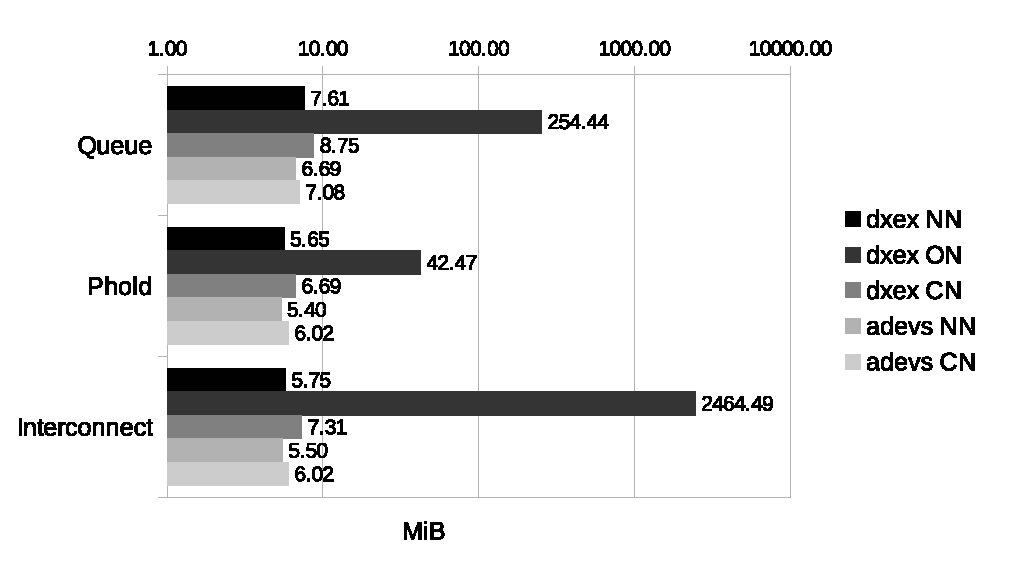
\includegraphics[width=\columnwidth]{fig/memory_voorlopig.eps}
    \caption{Memory usage results.}
    \label{fig:memory}
\end{figure}


% CONCLUSION
\subsection{Conclusion}
We have shown that our contribution is invaluable for high performance simulation: depending on the expected behaviour, modellers can choose the most appropriate synchronization protocol.
We will summarize the key aspects in achieving good parallel performance here. % reword aspects syn
\subsubsection{Allocation}
Allocation of atomic models over kernels is critical to obtain a speedup. 
In the case of the Interconnect model it is not possible to allocate models without introducing a cyclic dependency between kernels with severe performance degradation as a result. 
Even when no cycles exist in the topology between kernels a good allocation scheme will minimize the number of connections between kernels and aim for a star topology as in PHoldTree with depth first allocation or a chain topology as in the Queue model. 
Dxex can optionally offer the user a visualization of the behaviour of the kernels under a user supplied allocation scheme to allow for more insight. 
The same instrumentation could in future be used to optimize an existing allocation scheme.
\subsubsection{Uncertainty}
A simulation where future behaviour cannot be predicted is typically not suited for conservative simulation, but we have demonstrated that dxex's conservative kernel can still offer a non trivial speedup in this context. 
Optimistic is not constrained by this uncertainty and can offer a good speedup regardless of lookahead. 
Phold and PholdTree demonstrate that a single model can benefit from different synchronization protocols depending on a single parameter.
\subsubsection{Limits}
Dxex's conservative kernel is constrained by the amount of models it controls, as shown in the PHoldTree benchmark. This is especially the case when the minimal lookahead is $\epsilon$ requiring near constant polling of models for lookahead values. 
Optimistic is not constrained by the number of models it manages, but can quickly consume all available memory in a simulation. While this effect can be reduced with a thread aware allocation scheme, the underlying problem remains.




\section{Runtime Switching}
\label{sec:4b-hotswap}
Simply because a synchronization protocol is ideal at the start of the simulation, does not mean that it stays ideal during the simulation.
It is well known, and repeated in the previous section, that model behaviour significantly influences the ideal synchronization protocol.
Contrary to many modelling formalisms, the \textsf{DEVS} formalisms makes it possible to model basically any kind of discrete event model.
As such, it is possible for the model to significantly change its behaviour throughout the simulation.

Defining the ideal synchronization protocol at the start of the simulation, when information about future model behaviour is scarce, might therefore not offer the best possible performance.
In \textit{dxex}, we not only make it possible to define the synchronization protocol to use, but also to change this decision throughout simulation.
To do this, all kernels are notified of the switch and they are forced to stop simulation.
When stopped, each kernel instantiates a new core, with the new synchronization protocol, that is provided with the simulation state of the previous core.
Simulation is then resumed with the new cores after the previous ones are destroyed.

As usual, switching imposes an overhead and should thus only be done if the benefits outweigh the induced overhead.
This overhead depends on the size of the model and the number of simulation cores.
For a simple model and a few cores, the overhead is less than a second.

Although we currently only support manual switches between different synchronization protocols, this is not necessarily the case.
Ideally, a new component is added to the simulation kernel, which monitors model behaviour and simulation performance, and toggles between them automatically.
Our interface is augmented with the necessary bindings for such a decision component.
Also, our interface is augmented with an interface for statistics gathering and model behaviour analysis.
With all interfaces implemented and tested, we only leave open the actual switching logic.
Machine learning is a possible direction for future implementations of this decision component.

\subsection{Statistics Gathering}
Traditionally, models are not exposed to simulation kernel details as they work at a different level of abstraction:
simulation models only care about simulation results, and not about how these results are obtained (\textit{e.g.}, through parallel or distributed simulation).
This is different for a new simulation kernel component that has to monitor the behaviour of not only the model, but the simulator as well.

We add performance metrics in the simulation kernel, which logs relevant performance metrics and processes them for use in other components.
These metrics include the number of events created and destroyed, the number of inter- and intra-kernel events, the number of rollbacks, the measured lookahead, details of the GVT and EOT calculations, and information on the fairness between simulation kernels.
With all these metrics, the decision component can get a global view on both model and simulation kernel behaviour.

For example, if the actually seen lookahead is significantly higher than the defined lookahead, it might be interesting to switch to optimistic synchronization.
When the number of rollbacks is excessively high, switching to conservative synchronization might be considered.

\subsubsection{Visualization of Communication}
To provide more insight in our benchmark models, we created a simple visualization of their simulation trace.
This trace visualizes the allocation of the model and all defined connections.
For each connection, the number of events transferred is annotated.
Examples are shown for the three benchmark models used before: Figure~\ref{fig:Queue_allocation}, Figure~\ref{fig:interconnect_allocation_parallel}, and Figure~\ref{fig:phold_allocation} show traces for the Queue, Interconnect, and PHOLD models, respectively.
Using this information, we notice that the Interconnect benchmark indeed has a lot of inter-kernel events.
Despite the similar structure, the PHOLD model does not have as many inter-kernel events.
These results are relevant information that can be used by the hotswapping component.

\begin{figure*}
    \center
    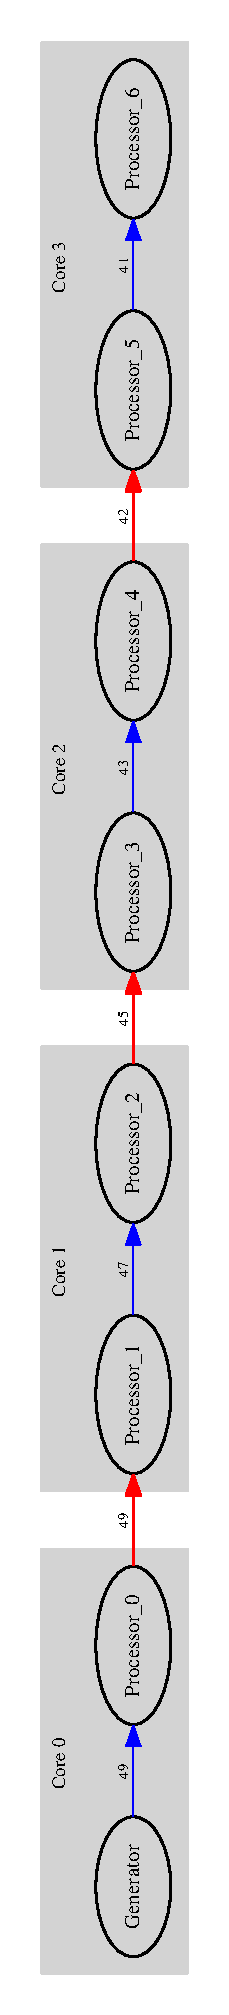
\includegraphics[height=\textwidth, angle=-90 ]{fig/queue_allocation.eps}
    \caption{Queue model simulation trace across 4 kernels.}
    \label{fig:Queue_allocation}
\end{figure*}

\begin{figure}
    \center
    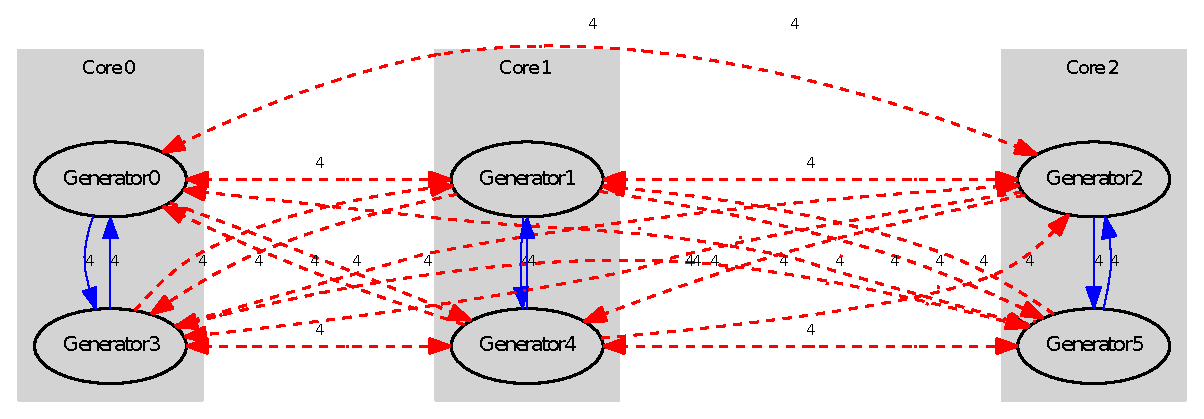
\includegraphics[width=\plotfraction\columnwidth]{fig/interconnect_parallel_allocation.eps}
    \caption{Interconnect simulation trace for 6 models on 3 kernels.}
    \label{fig:interconnect_allocation_parallel}
\end{figure}

\begin{figure}
    \center
    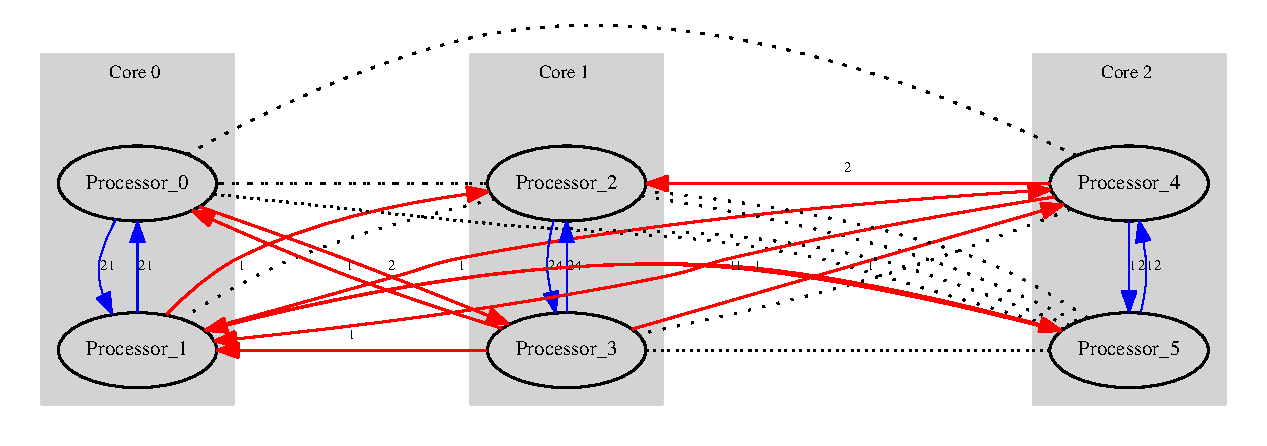
\includegraphics[width=\plotfraction\columnwidth]{fig/phold_parallel_allocation.eps}
    \caption{Phold simulation trace for parallel simulation using three kernels.}
    \label{fig:phold_allocation}
\end{figure}


\section{Model Allocation}
\label{sec:4a-allocation}
Although the synchronization protocol is one of the defining factors in simulation performance, model allocation has a significant impact on which protocol is ideal.
Depending on the model structure, and how it is mapped to the different kernels, it might not even make sense to parallelize at all.
Indeed, if the model is allocated such that frequent communication is necessary between kernels, parallelism is naturally reduced.
This brings us to the topic of model allocation, as also implemented in \textit{PythonPDEVS}~\cite{PythonPDEVS2}.

The modeller can specify which kernel a model should be allocated to, should such manual intervention be required.
This is handled by the default model allocator.
If no preference is given, a simple striping scheme is used but this is often insufficient.
By overriding the default allocator, a modeller tunes the allocation scheme for a specific model, maximizing multi core speedup.
This interface can be linked to graph algorithms for automatic allocation scheme generation, for example to avoid cycles in the dependency graph.

\subsection{Performance Evaluation}
To evaluate the influence of model allocation, we define a new model, based on PHOLD~\cite{PHOLD}.
The model structure resembles a tree: an atomic model can have a set of children, with children being connected to each other recursively.

Unlike the Queue model, the width of the hierarchy is still present in the topology of the atomic models after direct connection.
The PHOLDTree model allows us to investigate multi core speedup in terms of model allocation, by modifying the depth and width (fanout) model parameters.

The PHOLDTree model is similar in structure to models of gossiping in social networks~\cite{Gossip}.
The lookahead of an atomic node is the minimally allowed $\epsilon$, as is often the case in realistic models (\textit{e.g.}, if it is unknown what the lookahead might be).
We demonstrate the importance of allocation by comparing performance of a breadth-first versus a depth-first scheme.
Both options are automated ways of allocation that are independent of the model.

\begin{figure}
    \center
    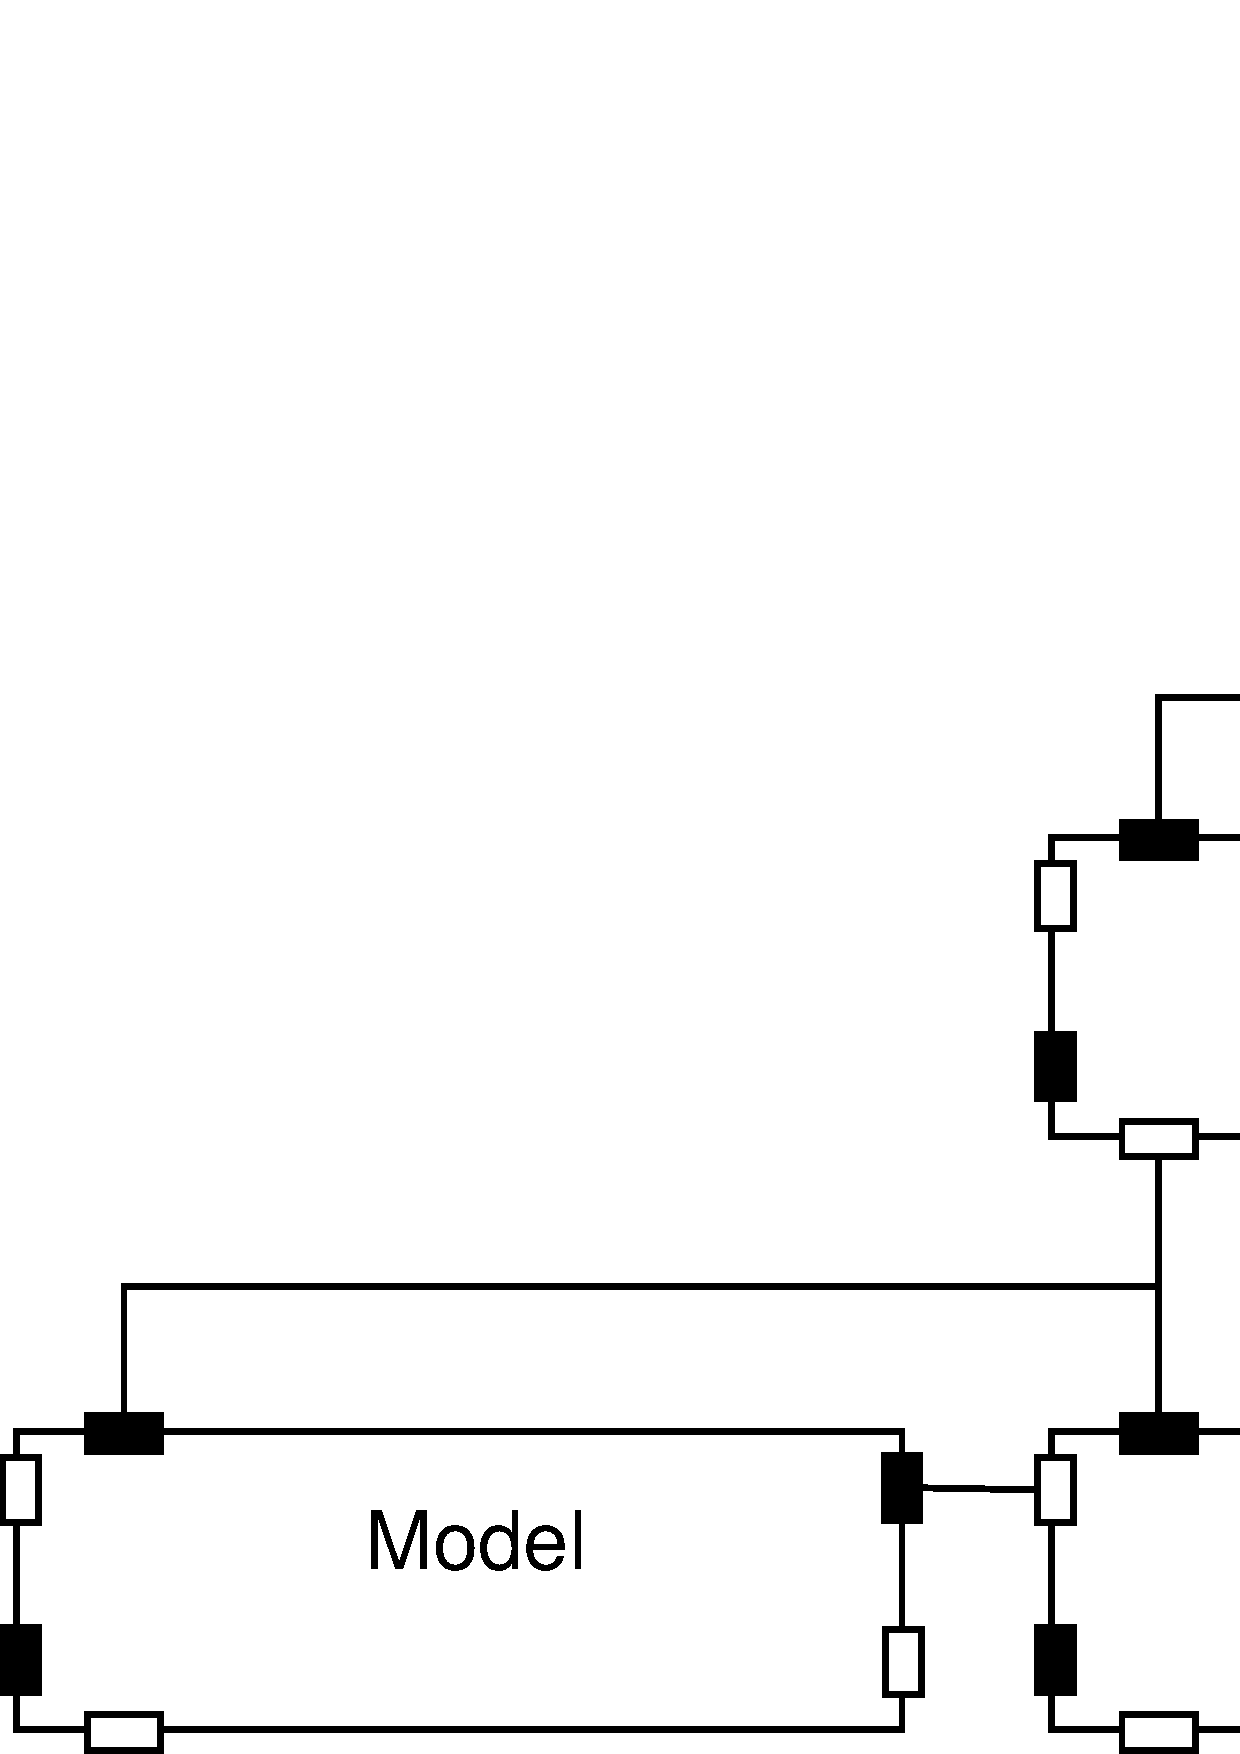
\includegraphics[width=\columnwidth]{fig/pholdtree.pdf}
    \caption{PHOLDTree model for depth 3 and width 2.}
    \label{fig:PHOLDTree_model}
\end{figure}

PHoldtree, like Queue, is a highly hierarchical model but one where the flattened structure cannot be partitioned into a chain, as was the case in the Queue model.
This topology is interesting since it highlights the effects of allocation.
First, we evaluate the model in single core simulation to provide a baseline for parallel simulation.

\subsubsection{Single Core Simulation}
Since \textit{adevs} does not use direct connection, we expect a noticeable performance difference between \textit{dxex} and \textit{adevs}.
This is shown in Figure~\ref{fig:PHOLDtree_seq_dn_benchmark}, where the fanout ($n$) determines the performance penalty \textit{adevs} suffers compared to \textit{dxex}.
Profiling indeed indicates that an increase in width per subtree ($n$) leads to higher overheads in \textit{adevs} due to the lack of direct connection.
\textit{Dxex} uses direct connection, making it independent of fanout.
Performance of \textit{dxex} is, in this model, only dependent on the number of models.
Slight deviations can still be seen, though, caused by the initialization overhead of direct connection.
Both \textit{adevs} and \textit{dxex} scale linearly in the number of atomic models.

\begin{figure}
    \center
    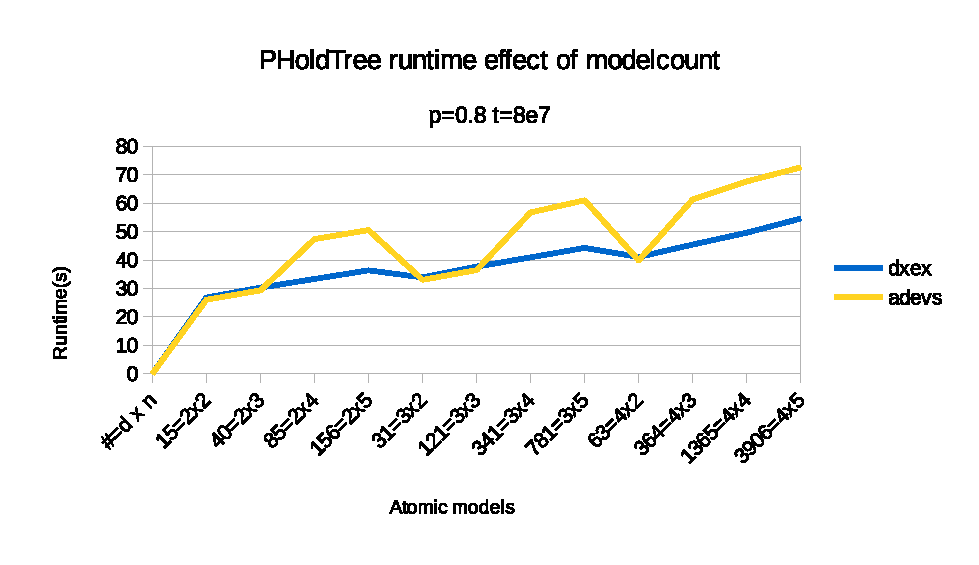
\includegraphics[width=\columnwidth]{fig/pholdtree_sequential_dn.eps}
    \caption{Effect of hierarchy in single core simulation.}
    \label{fig:PHOLDtree_seq_dn_benchmark}
\end{figure}

\subsubsection{Multi Core Simulation}
Next, we run the model using two different model allocation schemes: breadth-first and depth-first.
But first, we explain what we mean by both allocation schemes.

With breadth-first allocation, we traverse the tree in a breadth-first way, allocating subsequently visited atomic models to the same node.
This means, intuitively, that atomic models at the same level in the tree, but not necessarily siblings, are frequently allocated to the same node.
Since there is only infrequently some communication between siblings, and even never between different subtrees, this does not sound an intuitive allocation.
This allocation strategy is shown in Figure~\ref{fig:PholdTree_model_bfs}.

\begin{figure}
   \center
   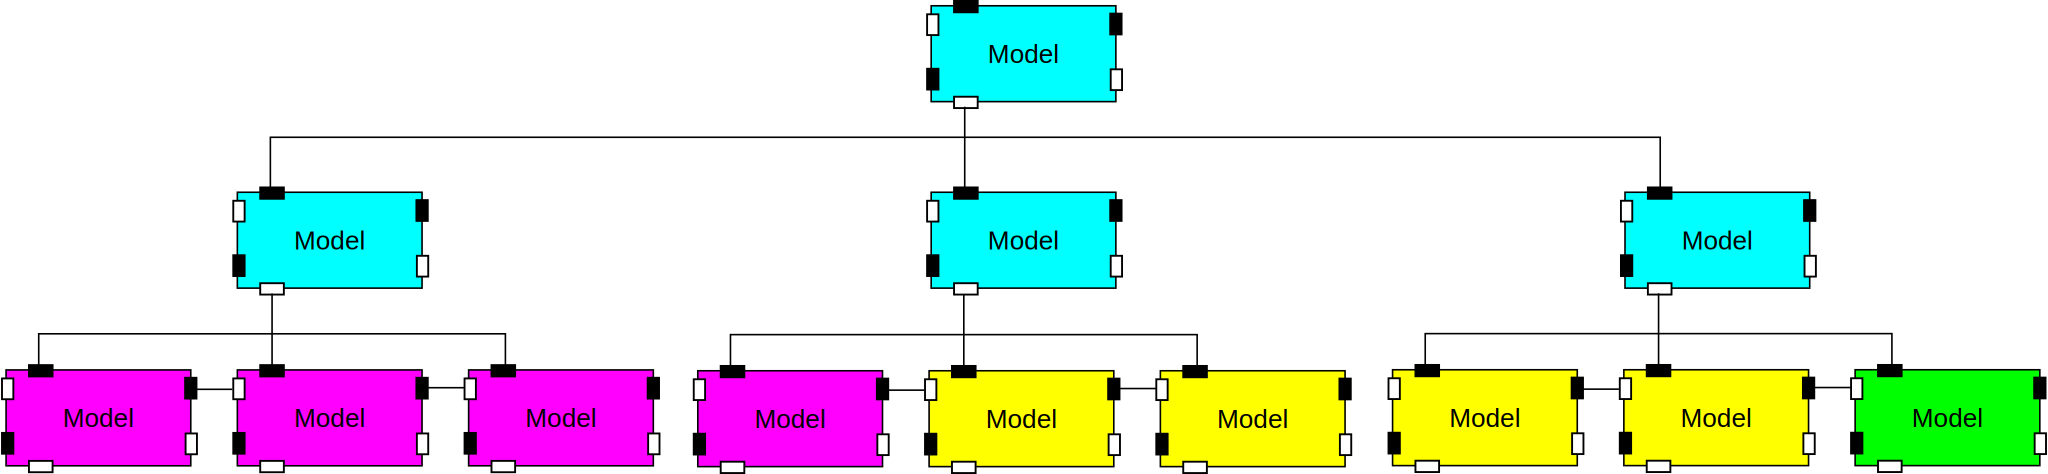
\includegraphics[width=\columnwidth]{fig/pholdtree_alloc_BF.pdf}
   \caption{PHOLDTree model breadth first allocation with 4 kernels.}
   \label{fig:PholdTree_model_bfs}
\end{figure}

With depth-first allocation, we traverse the tree in a depth-first way, allocating subsequently visited atomic models to the same node.
This means, intuitively, that subtrees are frequently allocated to the same node.
This allocation strategy is shown in Figure~\ref{fig:PholdTree_model_dfs}.

\begin{figure}
   \center
   \includegraphics[width=\columnwidth]{fig/pholdtree_alloc_DF.pdf}
   \caption{PHOLDTree model depth first allocation with 4 kernels.}
   \label{fig:PholdTree_model_dfs}
\end{figure}

Both allocators will try to divide models evenly over kernels.
The effects of varying the number of models per kernel are already evaluated in the previous section on scaling.
Here we want to highlight the overhead of communication and inter-kernel dependence. 

The breadth first allocation scheme results in a dependency chain with multiple branches, much like in the Queue model.
Such a linear dependency chain can result in a multi core speedup as we demonstrated with the Queue model.
This is not always true though: a single kernel with an unbalanced number of atomic models or unequal computational load in transition functions slows down the remainder of the chain.
This effect is also apparent if the thread a kernel runs on is not fairly scheduled.
With conservative synchronization this leads to excessive polling of the EOT of the other kernels.
With optimistic synchronization this leads to a cascade of rollbacks, since dependent kernels will simulate ahead of the slower kernel.

After simulation the traces can be visualized for both breadth-first and depth-first allocation.
Using a breadth-first allocation scheme, as shown in Figure~\ref{fig:pholdtree_visualize_parBFS}, we notice that many events get exchanged between kernels.
This is caused by the high number of inter-kernel connections and the high number of events exchanged over these connections.
The number of connections between nodes at the same simulation kernel is also rather low.
Using a depth-first allocation scheme, however, as shown in Figure~\ref{fig:pholdtree_visualize_parDFS}, minimizes inter-kernel connections while maximizing intra-kernel connections.

\begin{figure}
    \center
    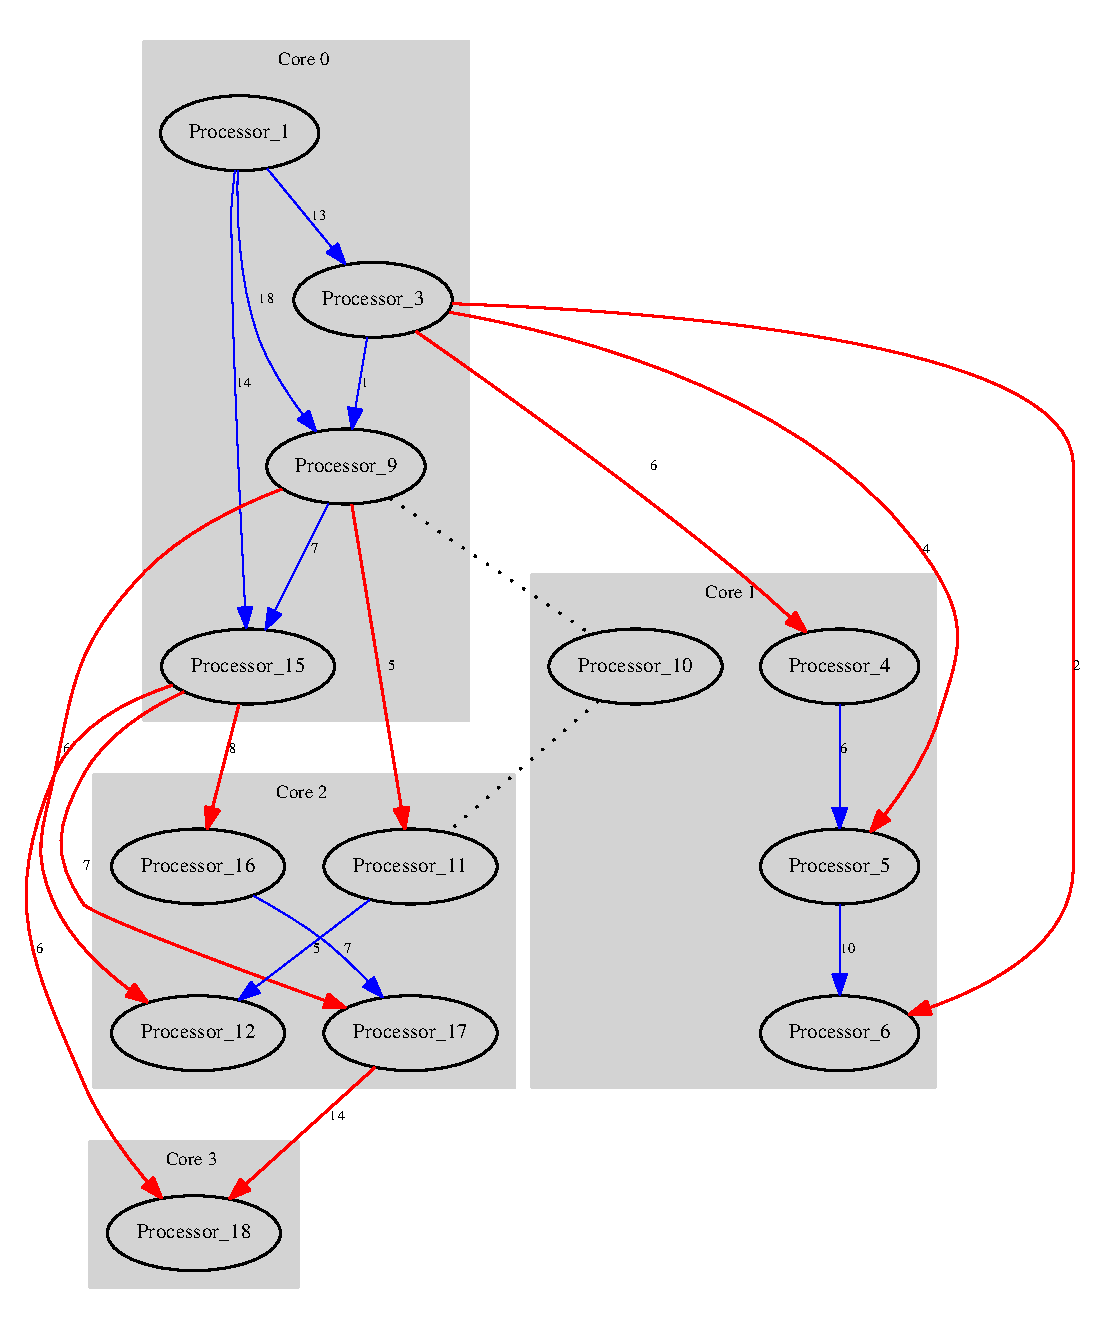
\includegraphics[width=\columnwidth]{fig/pholdtreed1n3t5000c4BFS.eps}
    \caption{Visualization of a simulation of the model in Figure~\ref{fig:PholdTree_model_bfs}.}
    \label{fig:pholdtree_visualize_parBFS}
\end{figure}

\begin{figure}
    \center
    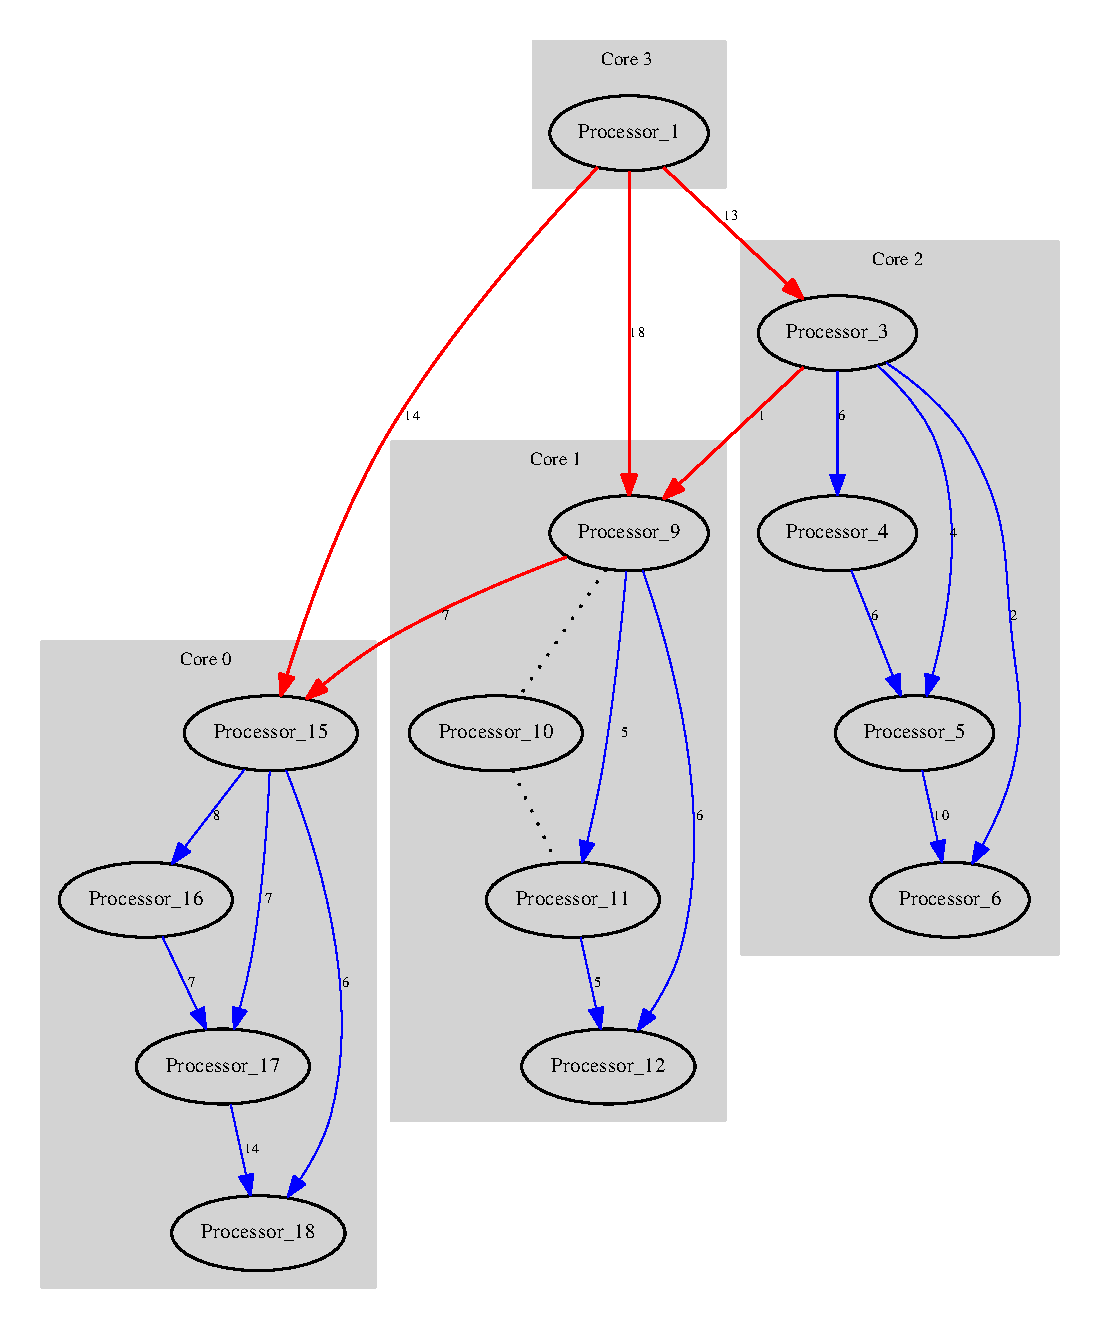
\includegraphics[width=\columnwidth]{fig/pholdtreed1n3t5000c4DFS.eps}
    \caption{Visualization of a simulation of the model in Figure~\ref{fig:PholdTree_model_dfs}.}
    \label{fig:pholdtree_visualize_parDFS}
\end{figure}

Simulation results are shown in Figure~\ref{fig:PholdTree_plot_alloc_high} for both allocation schemes in combination with both synchronization protocols.
We see that for both synchronization protocols, the depth-first allocation is significantly better than breadth-first allocation.
This is what we expected for this model: depth-first allocation maintains locality better than breadth-first allocation.
Whereas this is the case in this example, this is not true in general, as the ideal allocation depends on the model being simulated.

The most prominent aspect of these results is the low performance for conservative depth-first allocation for two kernels.
This is mostly caused by the difference between a single core simulation and a multi core simulation: suddenly we need to take into account synchronization and passing around of lookahead values.
And since the number of kernels is low, the overhead dominates any further speedup.
Optimistic is less sensitive to the number of models per kernel as it does not need to poll each model for a lookahead, this explains the lower runtime penalty observed for optimistic.

%The effect is due to the topology of the kernels, in BFS the risk on reverts is higher. Optimistic is less influenced but will get a lower speedup in the good case.
Interestingly, we see that optimistic synchronization is less influenced by the allocation than conservative synchronization.
This is likely caused by the lower number of connections to take into account in conservative synchronization.
Whereas conservative synchronization needs to take into account even scarcely used connections, optimistic synchronization does not.
The same is true in the opposite direction, though, where optimistic synchronization is slower when a good allocation is chosen.
Conservative synchronization will then be able to make better estimates, whereas optimistic synchronization does not make estimations. 

\begin{figure}
    \center
    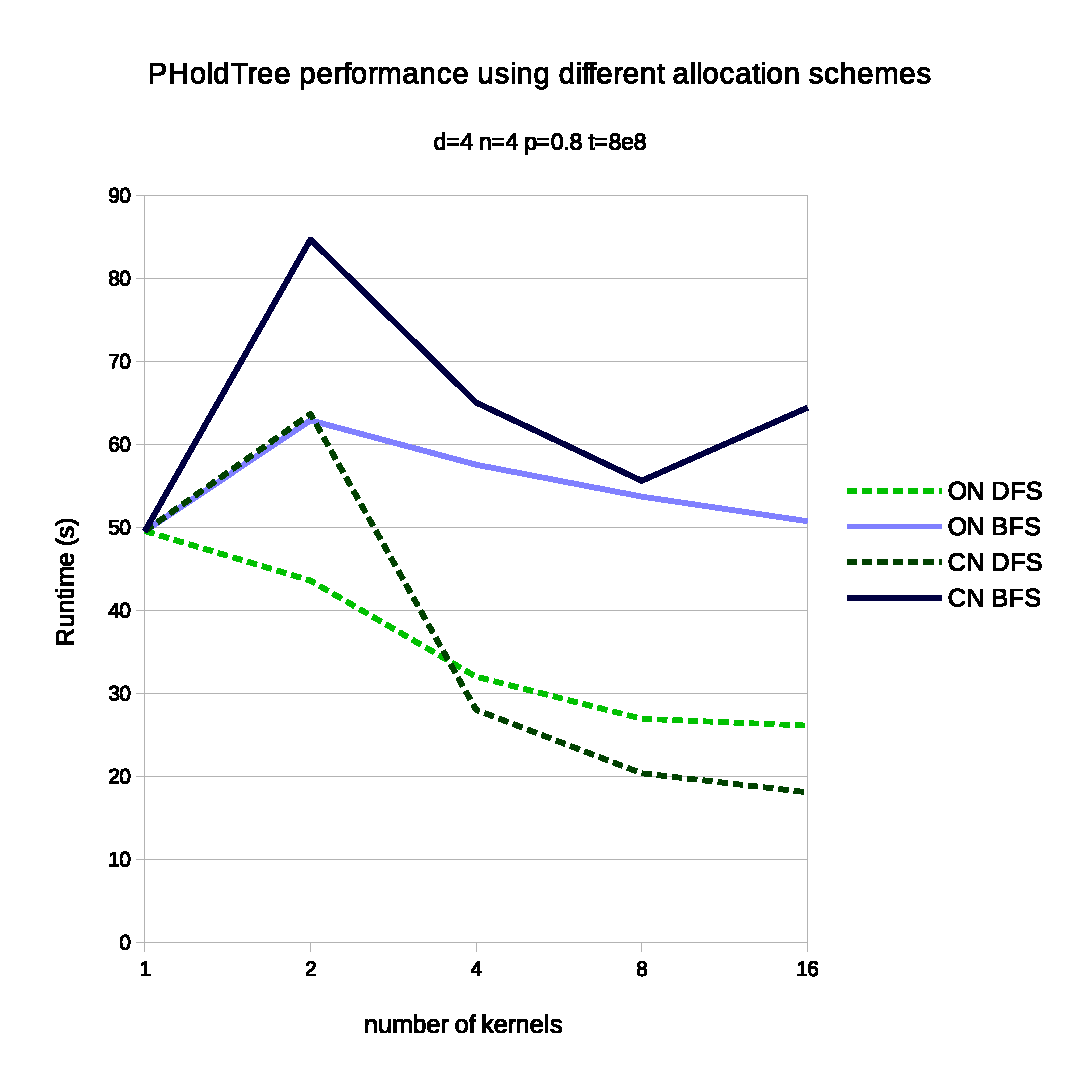
\includegraphics[width=\columnwidth]{fig/pholdtreeallochighp.eps}
    \caption{PHOLDTree model performance using different allocation schemes.}
    \label{fig:PholdTree_plot_alloc_high}
\end{figure}


\section{Related Work}
\label{sec:5-related-work}
Several similar \textsf{DEVS} simulation tools have already been implemented, though they differ in several key aspects.
We discuss several dimensions of related work, as we try to compromise between different tools.

In terms of code design and philosophy, dxex is most related to PythonPDEVS~\cite{PythonPDEVS}.
Performance of PythonPDEVS was still decent through the use of ``hints'' from the modeler.
In this spirit, we offer users the possibility to choose between different synchronization protocols.
This allows users to choose the most appropriate synchronization protocol, depending on the model.
Contrary to PythonPDEVS, however, dxex doesn't support distributed simulation~\cite{JDF}, model migrations~\cite{PythonPDEVS2}, or activity hints~\cite{PythonPDEVS_ACTIMS}.

Although PythonPDEVS offers very fast turnaround cycles, simulation performance was easily outdone by compiled simulation kernels.
In terms of performance, adevs~\cite{adevs} offered much faster simulation, at the cost of a significant compilation time.
The turnaround cycle in adevs is much slower though, specifically because the complete simulation kernel is implemented using templates in header files.
As a result, the complete simulation kernel has to be compiled again every time.
Similarly to vle~\cite{vle} and PowerDEVS~\cite{PowerDEVS}, dxex compromises by separating the simulation kernel into a shared library.
After the initial compilation of the simulation tool, only the model has to be compiled and linked to the shared library.
This significantly shortens the turnaround cycle, while still offering good performance.
In terms of performance, dxex is shown to be competitive with adevs.
Despite its high performance, adevs does not support optimistic synchronization, which we have shown to be highly relevant.

Previous \textsf{DEVS} simulation tools have already implemented multiple synchronization protocols, though none have done it in a strictly modular way that allows straightforward protocol switching for a single given model.
For example, adevs only supports conservative synchronization, and vle only supports experiment-level parallelism (\textit{i.e.}, run multiple experiments concurrently).
Closest to our support for multiple synchronization protocols is CD++~\cite{CD++}.
For CD++, both a conservative (CCD++~\cite{CCD++}) and optimistic (PCD++)~\cite{PCD++}) variant exist.
Despite the implementation of both protocols, they are different projects entirely.
Some features might therefore be implemented in CCD++ and not in PCD++, or vice versa.
And while this might not yet be that significant a problem to this day, this problem will only get worse when each project follows its own course.
Dxex, on the other hand, is a single project, where the choice of synchronization protocol is a simple configuration.
CD++, however, implements both conservative and optimistic synchronization for distributed simulation, whereas we limit ourselves to parallel simulation.
By limiting our approach to parallel simulation, we are able to achieve higher speedups through the use of shared memory communication.

In the PDES community, the problem of choosing between synchronization protocols is well known and documented~\cite{Jha:1994:UFC:195291.182480}.
The challenges of implementing such runtime switching have previously been explored already~\cite{Das:1996:APP:256562.256602}, and an implementation was given by, for example~\cite{perumalla2005musik}.
Our contribution entails bringing this same feature to the DEVS community, further expanding upon our unique feature of multiple synchronization protocols.

Model allocation and its impact on parallel performance has previously also been studied in the PDES community~\cite{PDESpartitioning}.
Referenced as partitioning of the simulation model, most studies distinguish between communication overhead and computational distribution (load balancing) as the two dimensions to partition over.
Partitioning a simulation model is identified as an issue to achieve scalability~\cite{Scalability}. 
Some research in the context of Parallel DEVS has been done, where they turn their attention to load balancing and communication overhead~\cite{PDEVSpartitioning}.
Our contribution studies the effect of partitioning with emphasis on the effect of communication between processes and in the presence of a flattened hierarchy. 
We focus on static partitioning since this is a limiting factor for our conservative synchronization implementation which does not support model relocation.
Model relocation, as implemented by PythonPDEVS~\cite{PythonPDEVS2}, might be an interesting addition to only model allocation at the start of simulation.

In summary, dxex tries to find the middle ground between the concepts of PythonPDEVS, the performance of adevs, and the multiple synchronization protocols of CD++.
To further profit from our multiple synchronization protocols in a single tool, we further added runtime switching between synchronization protocols and model allocation support.


\section{Conclusions and Future Work}
\label{sec:6-conclusion}
In this paper, we introduced \textit{DEVS-Ex-Machina} (``\textit{dxex}''), a new C++11-based \textsf{Parallel DEVS} simulation tool.
Our main contribution is the implementation of multiple synchronization protocols for parallel multicore simulation.
We have shown that there are indeed models which can be simulated significantly faster using either synchronization protocol.
\textit{Dxex} allows the user to choose between either conservative or optimistic synchronization at the start of simulation.
Depending on observed model behaviour and simulation performance, runtime switching between synchronization protocols can be used.

Notwithstanding our modularity, \textit{dxex} achieves performance competitive to \textit{adevs}, another very efficient \textsf{DEVS} simulation tool.
Performance is measured both in elapsed time, and memory usage.
Our empirical analysis shows that allocation of models over kernels is critical to enable a parallel speedup. Furthermore we have shown when and why optimistic synchronization can outperform conservative and vice versa. Finally we investigated the effect of memory (de)allocation on parallel simulation. 

Future work is possible in several directions.
First, our implementation of optimistic synchronization should be more tolerant to low-memory situations.
In its current state, simulation will simply halt with an out-of-memory error. The use of transactional memory can offer several advantages in this project. If it becomes part of the new C++17 standard it would be of great interest to see if it can help reduce the performance effects of memory allocation and synchronization.
Having simulation control, which can throttle the speed of nodes that use up too much memory, has been shown to work in these situations~\cite{FujimotoBook}.
Faster GVT implementations~\cite{Fujimoto:1997:CGV:268403.268404,Bauer:2005:SND:1069810.1070159} might further help to minimize this problem.
Second, the runtime switching between synchronization protocols can be driven using machine learning techniques.
The simulation engine is already capable of collecting data to inform such a process, and is designed to listen for commands from an external component.
Third, automatic allocation might be possible by analysis of the connections between models.
This information is already used in \textit{dxex} to construct the dependency graph in conservative synchronization.
A graph algorithm that distributes models, while avoiding cycles, could be used to offer a parallel speedup in either optimistic or conservative synchronization.
Similarly, it could serve as a default parallel allocation scheme that can be improved by the user.


\section*{ACKNOWLEDGMENTS}
This work was partly funded with a PhD fellowship grant from the Research Foundation - Flanders (FWO). 
Partial support by the Flanders Make strategic research centre for the manufacturing industry is also gratefully acknowledged.

\bibliographystyle{SageV}
\bibliography{papers}

\end{document}
